\documentclass[a4paper, openany]{memoir}

\usepackage[utf8]{inputenc}
\usepackage[T1]{fontenc} 
\usepackage[english]{babel}
\usepackage{fancyhdr}
\usepackage{float}
\usepackage{amsmath}
\usepackage{amsthm}
\usepackage{amssymb}
\usepackage{enumitem}
\usepackage[bookmarksopen=true,bookmarksopenlevel=2]{hyperref}
\usepackage{tikz}
\usepackage{pgfplots}
\usepackage{indentfirst}
\usepackage{bm}

\pagestyle{fancy}
\fancyhf{}
\fancyhead[LE]{\leftmark}
\fancyhead[RO]{\rightmark}
\fancyhead[RE, LO]{3H MSBT}
\fancyfoot[LE, RO]{\thepage}
\fancyfoot[RE, LO]{Pete Gautam}

\renewcommand{\headrulewidth}{1.5pt}

\theoremstyle{definition}
\newtheorem{definition}{Definition}[section]

\theoremstyle{plain}
\newtheorem{theorem}[definition]{Theorem}
\newtheorem{lemma}[definition]{Lemma}
\newtheorem{proposition}[definition]{Proposition}
\newtheorem{corollary}[definition]{Corollary}
\newtheorem{example}[definition]{Example}

\chapterstyle{thatcher}
% \setcounter{chapter}{2}
\pgfplotsset{compat=newest}

\begin{document}
\chapter{Metric Spaces}
\section{Introduction to Metric Spaces}
\subsection{Definition of a Metric Space}
In this section, we will define a metric space.
\begin{definition}
Let $X$ be a set and $d: X \times X \to \mathbb{R}$ be a function. Then, $(X, d)$ is a \emph{metric space}\sidefootnote{If the function $d$ is clear, we just say that $X$ is a metric space.} if:
\begin{enumerate}[label=\textbf{M\arabic*}.]
    \item for all $x_1, x_2 \in X$, $d(x_1, x_2) \geqslant 0$, and $d(x_1, x_2) = 0$ if and only if $x_1 = x_2$; 
    \item for all $x_1, x_2 \in X$, $d(x_1, x_2) = d(x_2, x_1)$; and
    \item for all $x_1, x_2, x_3 \in X$,
    \[d(x_1, x_3) \leqslant d(x_1, x_2) + d(x_2, x_3).\]
\end{enumerate}
If $(X, d)$ is a metric space, then we say that $d$ a \emph{metric} on $X$.
\end{definition}
\noindent Essentially, a metric space is a set where we can `measure distance'- the function $d$ gives us the distance between two points in the set $X$.\sidefootnote{For this reason, we call $d$ the \emph{distance function}.} The final axiom is called the triangle inequality.

Now, we look at some examples of metric spaces. If $X = \mathbb{R}$ and $d(x, y) = |x - y|$, then $(X, d)$ is a metric space. This is because, 
\begin{enumerate}[label=\textbf{M\arabic*}.]
    \item for $x_1, x_2 \in \mathbb{R}$, $|x_1 - x_2| \geqslant 0$, and $|x_1 - x_2| = 0$ if and only if $x_1 - x_2 = 0$, i.e. $x_1 = x_2$;
    \item for $x_1, x_2 \in \mathbb{R}$, $|x_1 - x_2| = |-1| \cdot |x_2 - x_1| = |x_2 - x_1|$; and
    \item for $x_1, x_2, x_3 \in \mathbb{R}$, 
    \[|x_1 - x_3| = |x_1 - x_2 + x_2 - x_3| \leqslant |x_1 - x_2| + |x_2 - x_3|.\]
\end{enumerate}
\noindent We can extend this to $X = \mathbb{C}$ and $d(x, y) = |x - y|$- this is still a metric space since it satisfies the same properties as above.

We will now look at the sets that can be metric spaces. It turns out that every set can be a metric space. This is because there is always a metric on a given set, called the \emph{discrete metric}. To see this, let $X$ be a set, and define the function $d: X \times X \to \mathbb{R}$ by
\[d(x_1, x_2) = \begin{cases}
0 & x_1 = x_2 \\
1 & x_1 \neq x_2
\end{cases}.\]
This is a metric:
\begin{enumerate}[label=\textbf{M\arabic*}.]
    \item Clearly, the value of the distance is always non-negative. Moreover, for $x_1, x_2 \in X$, if $x_1 = x_2$, then $d(x_1, x_2) = 0$, and if $x_1 \neq x_2$, then $d(x_1, x_2) \neq 0$. 
    \item Also, for $x_1, x_2 \in X$, if $x_1 = x_2$, then
    \[d(x_1, x_2) = 0 = d(x_2, x_1),\]
    and if $x_1 \neq x_2$, then
    \[d(x_1, x_2) = 1 = d(x_2, x_1).\]
    \item Furthermore, the triangle inequality is satisfied. We prove this in two cases:
    \begin{itemize}
        \item For $x_1, x_2, x_3 \in X$, if $x_1 = x_3$, then
        \[d(x_1, x_3) = 0 \leqslant d(x_1, x_2) + d(x_2, x_3).\]
        
        \item Instead, for $x_1, x_2, x_3 \in X$, if $x_1 \neq x_3$, then we cannot have both $x_1 = x_2$ and $x_2 = x_3$. In that case,
        \[d(x_1, x_3) = 1 \leqslant d(x_1, x_2) + d(x_2, x_3).\]
    \end{itemize}
\end{enumerate}
So, it does not make sense to ask whether a set is a metric space- a set can have many metrics, e.g. $\mathbb{R}$ has the normal metric and the discrete metric.

Before looking at more examples, we prove Cauchy's inequality.
\begin{lemma}[Cauchy's Inequality]
Let $\bm{v}, \bm{w} \in \mathbb{R}^n$. Then,
\[\lvert \bm{v} \cdot \bm{w} \rvert \leqslant \lVert \bm{v} \rVert \cdot \lVert \bm{w} \rVert,\]
where $\lVert \bm{v} \rVert = \sqrt{\bm{v} \cdot \bm{v}}$.
\end{lemma}
\begin{proof}
Denote
\[\bm{v} = \begin{bmatrix}
v_1 & \dots & v_n
\end{bmatrix}, \qquad \bm{w} = \begin{bmatrix}
w_1 & \dots & w_n
\end{bmatrix}.\]
Define the function $f: \mathbb{R} \to \mathbb{R}$ by $f(\lambda) = (\bm{v} + \lambda \bm{w}) \cdot (\bm{v} + \lambda \bm{w})$. We know that $f(\lambda) \geqslant 0$ for all $\lambda \in \mathbb{R}$. We have
\[f(\lambda) = a \lambda^2 + b \lambda + c,\]
where $a = (\bm{w} \cdot \bm{w})$, $b = 2(\bm{v} \cdot \bm{w})$ and $c = (\bm{v} \cdot \bm{v})$. Since $f(\lambda) \geqslant 0$, we know that the equation has at most 1 (distinct) real solution. In that case, the discriminant $b^2 - 4ac \leqslant 0$. Therefore,
\begin{align*}
    b^2 &\leqslant 4ac \\
    4(\bm{v} \cdot \bm{w})^2 &\leqslant 4 (\bm{w} \cdot \bm{w})(\bm{v} \cdot \bm{v}) \\
    \lvert \bm{v} \cdot \bm{w} \rvert^2 &\leqslant \lvert \bm{v} \rvert^2 \cdot \lvert \bm{w} \rvert^2.
\end{align*}
This implies that $\lvert \bm{v} \cdot \bm{w} \rvert \leqslant \lVert \bm{v} \rVert \cdot \lVert \bm{w} \rVert$.
\end{proof}
\noindent Using this result, we can derive the Triangle inequality in $\mathbb{R}^n$.
\begin{proposition}
Let $\bm{v}, \bm{w} \in \mathbb{R}^n$. Then,
\[\lVert \bm{v} + \bm{w} \rVert \leqslant \lVert \bm{v} \rVert + \lVert \bm{w} \rVert.\]
\end{proposition}
\begin{proof}
By Cauchy's Inequality, we find that
\begin{align*}
    \lvert \bm{v} \cdot \bm{w} \rvert &\leqslant \lVert \bm{v} \rVert \cdot \lVert \bm{w} \rVert \\
    \lVert \bm{v} \rVert^2 + 2(\bm{v} \cdot \bm{w}) + \lVert \bm{w} \rVert^2 &\leqslant \lVert \bm{v} \rVert^2 + 2\lVert \bm{v} \rVert \cdot \lVert \bm{w} \rVert + \lVert \bm{w} \rVert^2 \\
    (\bm{v} + \bm{w}) \cdot (\bm{v} + \bm{w}) &\leqslant (\lVert \bm{v} \rVert + \lVert \bm{w} \rVert)^2 \\
    \lVert \bm{v} + \bm{w} \rVert &\leqslant \lVert \bm{v} \rVert + \lVert \bm{w} \rVert.
\end{align*}
\end{proof}
\noindent Now, we look at another example of a metric space. So, let $n \in \mathbb{Z}_{\geqslant 1}$, $X = \mathbb{R}^n$ and $d_2: \mathbb{R}^n \times \mathbb{R}^n \to \mathbb{R}$ by
\[d_2(\bm{x}, \bm{y}) = \lVert \bm{x} - \bm{y} \rVert = \sqrt{\sum_{i=1}^n (x_i - y_i)^2}.\]
We claim that $(\mathbb{R}^n, d_2)$ is a metric space. This is because:
\begin{enumerate}[label=\textbf{M\arabic*}.]
    \item For all $\bm{x}, \bm{y} \in \mathbb{R}^n$, $\lVert \bm{x} - \bm{y} \rVert \geqslant 0$. Moreover, if $\lVert \bm{x} - \bm{y} \rVert = 0$, then for all $i \in \{1, 2, \dots, n\}$, $x_i - y_i = 0$, and so $x_i = y_i$. This implies that $\bm{x} = \bm{y}$. That is, $\lVert \bm{x} - \bm{y} \rVert = 0$ if and only if $\bm{x} = \bm{y}$.
    
    \item For all $\bm{x}, \bm{y} \in \mathbb{R}^n$,
    \[d_2(\bm{x}, \bm{y}) = \sqrt{\sum_{i=1}^n (x_i - y_i)^2} = \sqrt{\sum_{i=1}^n (y_i - x_i)^2} = d_2(\bm{y}, \bm{x}).\]
    
    \item Moreover, for $\bm{x}, \bm{y}, \bm{z} \in \mathbb{R}^n$,
    \begin{align*}
        d_2(\bm{x}, \bm{z})^2 &= \lVert \bm{x} - \bm{z} \rVert^2 \\
        &= \lVert \bm{x} - \bm{y} + \bm{y} - \bm{z} \rVert \\
        &\leqslant \lVert \bm{x} - \bm{y} \rVert + \lVert \bm{y} - \bm{z} \rVert.
    \end{align*}
\end{enumerate}
The metric $d_2$ is called the \emph{Euclidean metric}- it measures the Euclidean distance in $\mathbb{R}^n$.

\subsection{Metrics on $\mathbb{R}^2$}
Now, we look at more metrics on $\mathbb{R}^2$. Let $d_1: \mathbb{R}^2 \times \mathbb{R}^2 \to \mathbb{R}$ be given by
\[d_1(\bm{x}, \bm{y}) = |x_1 - y_1| + |x_2 - y_2|,\]
where $\bm{x} = \begin{bmatrix}
x_1 & x_2
\end{bmatrix}, \bm{y} = \begin{bmatrix}
y_1 & y_2
\end{bmatrix}$. It turns out that $(\mathbb{R}^2, d_1)$ is a metric space. This is because:
\begin{enumerate}[label=\textbf{M\arabic*}.]
    \item for $\bm{x}, \bm{y} \in \mathbb{R}^2$, $d_1(\bm{x}, \bm{y}) \geqslant 0$. Moreover, if $d_1(\bm{x}, \bm{y}) = 0$, then $|x_1 - y_1| = |x_2 - y_2| = 0$. This implies that $\bm{x} = \bm{y}$. That is, $\lVert \bm{x} - \bm{y} \rVert = 0$ if and only if $\bm{x} = \bm{y}$.
    
    \item for all $\bm{x}, \bm{y} \in \mathbb{R}^2$,
    \[d_1(\bm{x}, \bm{y}) = |x_1 - y_1| + |x_2 - y_2| = |y_1 - x_1| + |y_2 - x_2| = d_1(\bm{y}, \bm{x}).\]
    
    \item for all $x, y, z \in \mathbb{R}^2$,
    \begin{align*}
        d_1(\bm{x}, \bm{z}) &= |x_1 - z_1| + |x_2 - z_2| \\
        &\leqslant |x_1 - y_1| + |y_1 - z_1| + |x_2 - y_2| + |y_2 - z_2| \\
        &= d_1(\bm{x}, \bm{y}) + d_1(\bm{y}, \bm{z}).
    \end{align*}
\end{enumerate}
The metric $d_1$ is called the \emph{taxicab metric} or the \emph{Manhattan metric}- it measures distance along straight lines. We illustrate this below.
\begin{figure}[H]
    \centering
    \begin{tikzpicture}
        \begin{axis}[
            axis lines=center, 
            ymin=-.5, ymax=4.5,
            xmin=-.5, xmax=4.5,
            xlabel=$x$, ylabel=$y$,
        ]
            \foreach \x in {1, 2, 3, 4} {
                \foreach \y in {1, 2, 3, 4} {
                    \edef\temp{\noexpand
                        \node[circle, draw, inner sep=1.5pt, blue, fill=blue!50, opacity=0.5] at (axis cs:\x,\y) {};
                    }\temp
                }
            };
            
            \draw[red, thick, ->] (1, 1.05) -- (1, 1.95);
            \draw[red, thick, ->] (1.05, 2) -- (1.95, 2);
            \draw[red, thick, ->] (2.05, 2) -- (2.95, 2);
            
            \draw[brown, thick, ->] (1.05, 1) -- (1.95, 1);
            \draw[brown, thick, ->] (2.05, 1) -- (2.95, 1);
            \draw[brown, thick, ->] (3, 1.05) -- (3, 1.95);
        \end{axis}
    \end{tikzpicture}
\end{figure}
\noindent Here, the distance between $(1, 1)$ and $(3, 2)$ is 3 since the $x$-coordinate changes by 2 and the $y$-coordinate changes by 1. We can generalise $d_1$ to $\mathbb{R}^n$ in the obvious way.

Now, let $d_\infty: \mathbb{R}^2 \times \mathbb{R}^2 \to \mathbb{R}$ be given by
\[d_\infty(\bm{x}, \bm{y}) = \max(|x_1 - y_1|, |x_2 - y_2|),\]
where $\bm{x} = \begin{bmatrix}
x_1 & x_2
\end{bmatrix}, \bm{y} = \begin{bmatrix}
y_1 & y_2
\end{bmatrix}$. It turns out that $(\mathbb{R}^2, d_\infty)$ is a metric space. This is because:
\begin{enumerate}[label=\textbf{M\arabic*}.]
    \item for $\bm{x}, \bm{y} \in \mathbb{R}^2$, $d_1(\bm{x}, \bm{y}) \geqslant 0$. Moreover, if $d_1(\bm{x}, \bm{y}) = 0$, then $\max(|x_1 - y_1|, |x_2 - y_2|) = 0$. So, $|x_1 - y_1| = |x_2 - y_2| = 0$. This implies that $\bm{x} = \bm{y}$. That is, $\lVert \bm{x} - \bm{y} \rVert = 0$ if and only if $\bm{x} = \bm{y}$.
    
    \item for all $\bm{x}, \bm{y} \in \mathbb{R}^2$,
    \[d_\infty(\bm{x}, \bm{y}) = \max(|x_1 - y_1|, |x_2 - y_2|) = \max(|y_1 - x_1|, |y_2 - x_2|) = d_\infty(\bm{y}, \bm{x}).\]
    
    \item for all $x, y, z \in \mathbb{R}^2$,
    \begin{align*}
        |x_1 - z_1| &\leqslant |x_1 - y_1| + |y_1 - z_1| \\
        &\leqslant \max(|x_1 - y_1|, |x_2 - y_2|) + \max(|y_1 - z_1|, |y_2 - z_2|),
    \end{align*}
    and
    \begin{align*}
        |x_2 - z_2| &\leqslant |x_2 - y_2| + |y_2 - z_2| \\
        &\leqslant \max(|x_1 - y_1|, |x_2 - y_2|) + \max(|y_1 - z_1|, |y_2 - z_2|).
    \end{align*}
    In that case,
    \begin{align*}
        d_\infty(\bm{x}, \bm{z}) &= \max(|x_1 - z_1|, |x_2 - z_2|) \\
        &\leqslant \max(|x_1 - y_1|, |x_2 - y_2|) + \max(|y_1 - z_1|, |y_2 - z_2|) \\
        &= d_\infty(\bm{x}, \bm{y}) + d_\infty(\bm{y}, \bm{z}).
    \end{align*}
\end{enumerate}
The metric $d_\infty$ is called the \emph{chessboard metric} or the \emph{Chebyshev metric}.

Next, we look at yet another metric on $\mathbb{R}^2$. Let $D: \mathbb{R}^2 \times \mathbb{R}^2 \to \mathbb{R}$ be given by
\[D(\bm{x}, \bm{y}) = \begin{cases}
d_2(\bm{x}, \bm{y}) & \bm{x}, \bm{y}, \bm{0} \text{ are collinear} \\
\lVert \bm{x} \rVert + \lVert \bm{y} \rVert & \text{otherwise}.
\end{cases}\]
Three points in $\mathbb{R}^2$ are said to be collinear if all three points lie on the same line. This is called the \emph{French Railroad metric}.

\subsection{Open Balls}
To see how a metric space behaves, we will consider open balls within a metric.
\begin{definition}
Let $(X, d)$ be a metric space, and let $x \in X$, $r \in \mathbb{R}_{> 0}$. Then, the \emph{open ball of radius $r$ about $x$} is the set
\[B_X(x, r) = \{y \in X \mid d(x, y) < r\}.\]
In particular, the \emph{unit ball} is $B_X(x, 1)$.
\end{definition}

We will illustrate the unit ball in $\mathbb{R}^2$ around the origin with different metrics:
\begin{itemize}
    \item taxicab metric $d_1$:
    \begin{figure}[H]
        \centering
        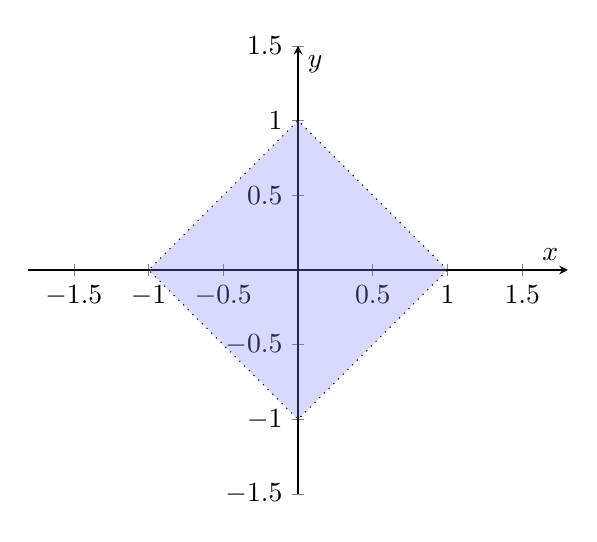
\begin{tikzpicture}
            \begin{axis}[
                axis lines=center, 
                ymin=-1.5, ymax=1.5,
                xmin=-1.5, xmax=1.5,
                xlabel=$x$, ylabel=$y$,
                xtick={1.5, 1, 0.5, 0, -0.5, -1, -1.5},
                ytick={1.5, 1, 0.5, 0, -0.5, -1, -1.5},
                axis equal,
            ]
            \fill[fill=blue!50, opacity=0.3] (axis cs:0,0) (1, 0) -- (0, 1) -- (-1, 0) -- (0, -1) -- (1, 0);
            \draw[dotted] (axis cs:0,0) (1, 0) -- (0, 1) -- (-1, 0) -- (0, -1) -- (1, 0);
            \end{axis}
        \end{tikzpicture}
    \end{figure}
    The unit ball around 0 is a rhombus since the sum of the $x$ and the $y$ coordinates must be less than 1.
    
    \item Euclidean metric $d_2$:
    \begin{figure}[H]
        \centering
        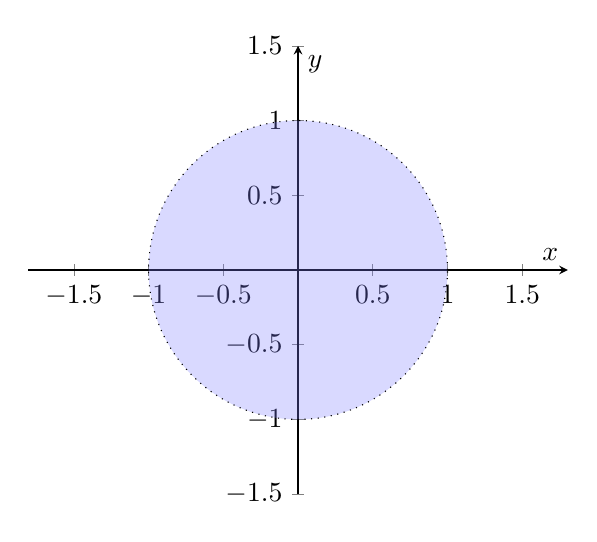
\begin{tikzpicture}
            \begin{axis}[
                axis lines=center, 
                ymin=-1.5, ymax=1.5,
                xmin=-1.5, xmax=1.5,
                xlabel=$x$, ylabel=$y$,
                xtick={1.5, 1, 0.5, 0, -0.5, -1, -1.5},
                ytick={1.5, 1, 0.5, 0, -0.5, -1, -1.5},
                axis equal,
            ]
                \fill[fill=blue!50, opacity=0.3] (axis cs: 0, 0) circle (1);
                \draw[dotted] (axis cs: 0, 0) circle (1);
            \end{axis}
        \end{tikzpicture}
    \end{figure}
    This is the usual unit ball around 0.
    
    \item chessboard metric $d_\infty$:
    \begin{figure}[H]
        \centering
        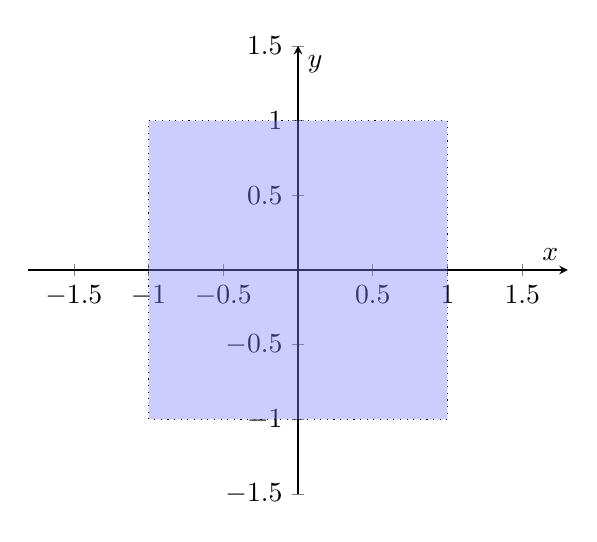
\begin{tikzpicture}
            \begin{axis}[
                axis lines=center, 
                ymin=-1.5, ymax=1.5,
                xmin=-1.5, xmax=1.5,
                xlabel=$x$, ylabel=$y$,
                xtick={1.5, 1, 0.5, 0, -0.5, -1, -1.5},
                ytick={1.5, 1, 0.5, 0, -0.5, -1, -1.5},
                axis equal,
            ]
                \fill[fill=blue!50, opacity=0.4] (axis cs:0,0) (1, 1) -- (1, -1) -- (-1, -1) -- (-1, 1) -- (1, 1);
                \draw[dotted] (axis cs:0,0) (1, 1) -- (1, -1) -- (-1, -1) -- (-1, 1) -- (1, 1);

            \end{axis}
        \end{tikzpicture}
    \end{figure}
    The unit ball around 0 is a square since the maximum value of the $x$ and the $y$ coordinates must be less than 1.
    
    \item the railroad metric:
    \begin{figure}[H]
        \centering
        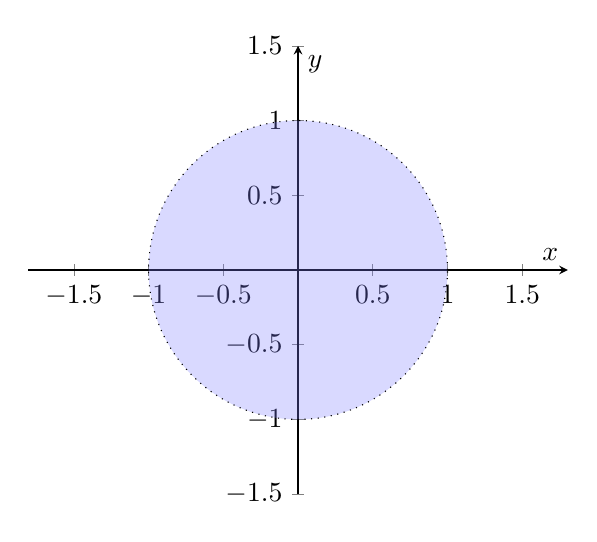
\begin{tikzpicture}
            \begin{axis}[
                axis lines=center, 
                ymin=-1.5, ymax=1.5,
                xmin=-1.5, xmax=1.5,
                xlabel=$x$, ylabel=$y$,
                xtick={1.5, 1, 0.5, 0, -0.5, -1, -1.5},
                ytick={1.5, 1, 0.5, 0, -0.5, -1, -1.5},
                axis equal,
            ]
                \fill[fill=blue!50, opacity=0.3] (axis cs: 0, 0) circle (1);
                \draw[dotted] (axis cs: 0, 0) circle (1);
            \end{axis}
        \end{tikzpicture}
    \end{figure}
    Here, the unit ball around the origin is the same for the Euclidean and the railroad metric. This is because, since we are considering the distance to the origin, the railroad distance is by definition equal to the Euclidean distance\sidefootnote{The points $\bm{0}, \bm{0}, \bm{x}$ are always collinear!}. The unit ball is around $(1, 1)$:
    \begin{figure}[H]
        \centering
        \begin{tikzpicture}
            \begin{axis}[
                axis lines=center, 
                ymin=-1.5, ymax=2.5,
                xmin=-1.5, xmax=2.5,
                xlabel=$x$, ylabel=$y$,
                xtick={2.5, 2, 1.5, 1, 0.5, 0, -0.5, -1, -1.5},
                ytick={2.5, 2, 1.5, 1, 0.5, 0, -0.5, -1, -1.5},
            ]
                \draw[ultra thick, blue!50, dotted] (axis cs:0,0) (0, 0) -- (2, 2);
            \end{axis}
        \end{tikzpicture}
    \end{figure}
    The unit ball is just the line interval from $(0, 0)$ to $(2, 2)$. If a point $\bm{x}$ does not lie in the interval, then the distance is
    \[D((1, 1), \bm{x}) = \lVert (1, 1) \rVert + \lVert \bm{x} \rVert \geqslant \sqrt{1^2 + 1^2} > 1,\]
    and so it cannot lie on the unit ball.
    
    \item the discrete metric:
    \begin{figure}[H]
        \centering
        \begin{tikzpicture}
            \begin{axis}[
                axis lines=center, 
                ymin=-1.5, ymax=1.5,
                xmin=-1.5, xmax=1.5,
                xlabel=$x$, ylabel=$y$,
                xtick={1.5, 1, 0.5, 0, -0.5, -1, -1.5},
                ytick={1.5, 1, 0.5, 0, -0.5, -1, -1.5},
            ]
                \filldraw[blue, opacity=0.5] (0, 0) circle (2pt);
            \end{axis}
        \end{tikzpicture}
    \end{figure}
    Only the value $0$ is in the open ball, since the distance to every other point from $0$ is $1$.
\end{itemize}

\subsection{Strong Equivalence}
We will now compare the metrics $d_1, d_2, d_\infty$.
\begin{lemma}
Let $\bm{x}, \bm{y} \in \mathbb{R}^2$. Then,
\begin{itemize}
    \item $d_\infty(\bm{x}, \bm{y}) \leqslant d_2(\bm{x}, \bm{y}) \leqslant d_1(\bm{x}, \bm{y})$;
    \item $d_1(\bm{x}, \bm{y}) \leqslant \sqrt{2} d_2(\bm{x}, \bm{y}) \leqslant 2 d_\infty(\bm{x}, \bm{y})$.
\end{itemize}
\end{lemma}
\begin{proof}
    Let $\bm{x} = \begin{bmatrix}
        x_1 & x_2
    \end{bmatrix}, \bm{y} = \begin{bmatrix}
        y_1 & y_2
    \end{bmatrix}$.
\begin{itemize}
    \item Without loss of generality, assume that $|x_1 - y_1| = \max(|x_1 - y_1|, |x_2 - y_2|)$. Then,
    \begin{align*}
        d_\infty(\bm{x}, \bm{y}) &= |x_1 - y_1| \\
        &= \sqrt{(x_1 - y_1)^2} \\
        &\leqslant \sqrt{(x_1 - y_1)^2 + (x_2 - y_2)^2} = d_2(\bm{x}, \bm{y}).
    \end{align*}
    Moreover,
    \begin{align*}
        0 &\leqslant 2 |x_1 - y_1| \cdot |x_2 - y_2| \\
        (x_1 - y_1)^2 + (x_2 - y_2)^2 &\leqslant |x_1 - y_1|^2 + 2|x_1 - y_1| \cdot |x_2 - y_2| + |x_2 - y_2|^2 \\
        (x_1 - y_1)^2 + (x_2 - y_2)^2 &\leqslant (|x_1 - y_1| + |x_2 - y_2|)^2 \\
        \sqrt{(x_1 - y_1)^2 + (x_2 - y_2)^2} &\leqslant |x_1 - y_1| + |x_2 - y_2|.
    \end{align*}
    This implies that $d_2(\bm{x}, \bm{y}) \leqslant d_1(\bm{x}, \bm{y})$.
    
    \item We find that
    \begin{align*}
        0 &\leqslant (|x_1 - y_1| - |x_2 - y_2|)^2 \\
        0 &\leqslant (x_1 - y_1)^2 - 2|x_1 - y_1| \cdot |x_2 - y_2| \\
        &+ (x_2 - y_2)^2 \\
        2|x_1 - y_1| \cdot |x_2 - y_2| &\leqslant (x_1 - y_1)^2 + (x_2 - y_2)^2 \\
        (x_1 - y_1)^2 & \\
        + 2|x_1 - y_1| \cdot |x_2 - y_2| + (x_2 - y_2)^2 &\leqslant 2 [(x_1 - y_1)^2 + (x_2 - y_2)^2] \\
        |x_1 - y_1| + |x_2 - y_2| &\leqslant \sqrt{2} \sqrt{(x_1 - y_1)^2 + (x_2 - y_2)^2} \\
        d_1(\bm{x}, \bm{y}) &\leqslant \sqrt{2} d_2(\bm{x}, \bm{y}). 
    \end{align*}
    Now, without loss of generality, assume that $|x_1 - y_1| = \max(|x_1 - y_1|, |x_2 - y_2|)$. In that case, 
    \begin{align*}
        |x_2 - y_2| &\leqslant |x_1 - y_1| \\
        2(x_2 - y_2)^2 &\leqslant 2(x_1 - y_1)^2 \\
        2[(x_1 - y_1)^2 + (x_2 - y_2)^2] &\leqslant 4(x_1 - y_1)^2 \\
        \sqrt{2} \sqrt{(x_1 - y_1)^2 + (x_2 - y_2)^2} &\leqslant 2|x_1 - y_1| \\
        \sqrt{2} d_2(\bm{x}, \bm{y}) &\leqslant d_\infty(\bm{x}, \bm{y}).
    \end{align*}
\end{itemize}
\end{proof}
\noindent The inequalities above tell us that these metrics are very similar- we define this similarity.
\begin{definition}
Let $d, d'$ be metrics on a set $X$. We say that $d, d'$ are \emph{strongly equivalent} if there exist $c_1, c_2 \in \mathbb{R}_{> 0}$ such that for all $x, y \in X$,
\[d(x, y) \leqslant c_1 d'(x, y) , \qquad d'(x, y) \leqslant c_1 d(x, y).\]
This is also denoted by \emph{Lipschitz equivalent}.
\end{definition}
\noindent Strong equivalence is an equivalence relation. 
\begin{proposition}
Let $X$ be a set. Define the relation $\sim$ on metrics of $X$ by
\[d_a \sim d_b \iff d_a \text{ and } d_b \text{ are strongly equivalent}.\]
Then, $\sim$ is an equivalence relation.
\end{proposition}
\begin{proof}
\hspace*{0pt}
\begin{itemize}
    \item Let $d$ be a metric on $X$. We know that for all $x, y \in X$,
    \[d(x, y) \leqslant d(x, y).\]
    Therefore, $d \sim d$.
    
    \item Let $d_a, d_b$ be metrics on $X$ such that $d_a \sim d_b$. In that case, there exist $c_1, c_2 \in \mathbb{R}_{> 0}$ such that for all $x, y \in X$,
    \[d_a(x, y) \leqslant c_1 d_b(x, y), \qquad d_b(x, y) \leqslant d_a(x, y).\]
    This implies that $d_b \sim d_a$.
    
    \item Let $d_a, d_b, d_c$ be metrics on $X$ such that $d_a \sim d_b$ and $d_b \sim d_c$. In that case, there exist $c_1, c_2, c_3, c_4 \in \mathbb{R}_{> 0}$ such that for all $x, y \in X$,
    \begin{align*}
        d_a(x, y) &\leqslant c_1 d_b(x, y), & d_b(x, y) &\leqslant c_2 d_a(x, y) \\
        d_b(x, y) &\leqslant c_3 d_c(x, y), & d_c(x, y) &\leqslant c_4 d_b(x, y).
    \end{align*}
    In that case,
    \[d_a(x, y) \leqslant c_1 d_b(x, y) \leqslant c_1 c_3 d_c(x, y),\]
    and
    \[d_c(x, y) \leqslant c_4 d_b(x, y) \leqslant c_4 c_2 d_a(x, y).\]
    So, $d_a \sim d_c$.
\end{itemize}
Therefore, $\sim$ is an equivalence relation.
\end{proof}

\noindent We will see later that `properties' in a metric space on a set only depend on the metric $d$ up to strong equivalence. We know that the metrics $d_1, d_2, d_\infty$ on $\mathbb{R}^2$ are strongly equivalent to each other.\sidefootnote{This can be extended to $\mathbb{R}^n$ for every $n \in \mathbb{Z}_{\geqslant 1}$.} 

It turns out that the railroad metric $D$ is not strongly equivalent on $\mathbb{R}^2$ to any of these metrics. We will show that $D$ is not strongly equivalent to $d_2$- since strong equivalence is an equivalence relation, it will follow that $D$ is not strongly equivalent to $d_1$ and $d_\infty$. So, assume for a contradiction that there exists a constant $c > 0$ such that $D(\bm{x}, \bm{y}) \leqslant cd_2(\bm{x}, \bm{y})$ for all $\bm{x}, \bm{y} \in \mathbb{R}^2$. We will define the sequences $(\bm{x}_n)_{n=1}^{\infty}$ and $(\bm{y}_n)_{n=1}^{\infty}$ in $\mathbb{R}^2$ by $\bm{x}_n = (n, 0)$ and $\bm{y}_n = (n, 1)$. Pictorially, we have the following:
\begin{figure}[H]
    \centering
    \begin{tikzpicture}
        \begin{axis}[
            axis lines=center, 
            ymin=-.5, ymax=1.5,
            xmin=-.5, xmax=7,
            xlabel=$x$, ylabel=$y$,
            xtick={6, 5, 4, 3, 2, 1},
            ytick={0, 1},
        ]
            \foreach \x in {1, 2, ..., 6} {
               \edef\temp{\noexpand
                    \node[circle, draw, inner sep=1.5pt, fill=blue!50, opacity=0.5] at (axis cs:\x,0) {};
                }\temp
                \edef\temp{\noexpand
                    \node[circle, draw, inner sep=1.5pt, fill=blue!50, opacity=0.5] at (axis cs:\x,1) {};
                }\temp
            };
        \end{axis}
    \end{tikzpicture}
\end{figure}
\noindent So, for any $n \in \mathbb{Z}_{\geqslant 1}$,
\[d_2(\bm{x}_n, \bm{y}_n) = \sqrt{(n-n)^2 + (0-1)^2} = 1,\]
and
\[D(\bm{x}_n, \bm{y}_n) = \lVert \bm{x}_n \rVert + \lVert \bm{y}_n \rVert = \sqrt{n^2 + 0^2} + \sqrt{n^2 + 1} \geqslant 2n.\]
since the points $\bm{x}_n, \bm{y}_n$ and $\bm{0}$ are not collinear. Therefore, for all $n \in \mathbb{Z}_{\geqslant 1}$,
\[2n \leqslant D(\bm{x}_n, \bm{y}_n) \leqslant cd_2(\bm{x}_n, \bm{y}_n) = c.\]
We can take $n > c$ to get a contradiction. Therefore, $D$ cannot be strongly equivalent to $d_2$.

\subsection{Subspace Metric}
We finish this section with subspace metric.
\begin{definition}
Let $(X, d)$ be a metric space, and let $A \subseteq X$. Define the function $d_A: A \times A \to \mathbb{R}$ given by $d_A(x, y) = d(x, y)$ for all $x, y \in A$. Then, we say that $(A, d_a)$ is a \emph{subspace metric}.
\end{definition}
We would want the subspace metric to be a metric space in its own right. It turns out that this is always the case. We check the axioms:
\begin{enumerate}[label=\textbf{M\arabic*}.]
    \item for all $x, y \in A$, $d_A(x, y) = d(x, y) \geqslant 0$, and $d_A(x, y) = d(x, y) = 0$ if and only if $x = y$;
    \item for all $x, y \in A$, $d_A(x, y) = d(x, y) = d(y, x) = d_A(y, x)$; and
    \item for all $x, y, z \in A$, 
    \[d_A(x, z) = d(x, z) \leqslant d(x, y) + d(y, z) = d_A(x, y) + d_A(y, z).\]
\end{enumerate}

\noindent Now, we consider examples of subspace metrics. Take $X = \mathbb{R}$, with the metric $d_2$. Then, $A = [-1, 1]$ is a subspace metric with a restriction of $d_2$ metric. Within this subspace, the open ball $B_A(-\frac{1}{2}, 1) = [-1, \frac{1}{2})$- the value $-1$ is included since $|\frac{1}{2} - 1| = \frac{1}{2} < 1$. This is not an open interval in $\mathbb{R}$. Moreover, $B_A(0, \frac{1}{2}) = (-\frac{1}{2}, \frac{1}{2})$- this is an open interval in $\mathbb{R}$. Finally, $B_A(1, 10) = [-1, 1]$- this is a closed interval in $\mathbb{R}$.

Next, take $X = \mathbb{R}^2$, with the metric $d_2$, and let $A = \{\bm{a}_1, \bm{a}_2, \bm{a}_2, \bm{a}_3, \bm{a}_4\}$, which are shown in the picture below.
\begin{figure}[H]
    \centering
    \begin{tikzpicture}
        \begin{axis}[
            axis lines=center, 
            ymin=-.5, ymax=3.5,
            xmin=-.5, xmax=3.5,
            xlabel=$x$, ylabel=$y$,
        ]
            
            \node[circle, draw, inner sep=1.5pt, blue, fill=blue!50, opacity=0.5, label={90:$\bm{a}_1$}] at (axis cs:1,0) {};
            \node[circle, draw, inner sep=1.5pt, blue, fill=blue!50, opacity=0.5, label={90:$\bm{a}_2$}] at (axis cs:2,0) {};
            \node[circle, draw, inner sep=1.5pt, blue, fill=blue!50, opacity=0.5, label={-90:$\bm{a}_3$}] at (axis cs:1,2) {};
            \node[circle, draw, inner sep=1.5pt, blue, fill=blue!50, opacity=0.5, label={-90:$\bm{a}_4$}] at (axis cs:2,2) {};
        \end{axis}
    \end{tikzpicture}
\end{figure}
\noindent In that case,
\begin{align*}
    d_A(\bm{a}_1, \bm{a}_2) &= 1, & d_A(\bm{a}_1, \bm{a}_3) &= 2, & d_A(\bm{a}_1, \bm{a}_4) &= \sqrt{5} \\
    d_A(\bm{a}_2, \bm{a}_3) &= \sqrt{5} & d_A(\bm{a}_2, \bm{a}_4) &= 2 & d_A(\bm{a}_3, \bm{a}_4) &= 1.
\end{align*}
Given the distances, it is difficult to check whether it is a metric space- realising a metric space as a subspace metric means we do not need to check for triangle inequality.
\newpage

\section{Function Spaces}
In this section, we will look at metric spaces on functions. Let $C[0, 1]$ be the space of all real-valued continuous functions $f: [0, 1] \to \mathbb{R}$. This is an infinite-dimensional vector space over $\mathbb{R}$. A metric $d_1: C[0, 1] \times C[0, 1] \to \mathbb{R}$ on this set is
\[d_1(f, g) = \int_0^1\left|f(x) - g(x)\right| \ dx.\]
This is the (unsigned) area between the two functions. We know that a continuous function is Riemann integrable, so the metric is well-defined. 

We will now verify that this $(C[0, 1], d_1)$ is a metric space. We start with a lemma.
\begin{lemma}
Let $h: [0, 1] \to \mathbb{R}$ be a continuous function such that there exists an $x_0 \in [0, 1]$ such that $h(x_0) = k > 0$. Then, there exists a $\delta > 0$ such that for $x \in [0, 1]$, if $|x - x_0| \leqslant \delta$, then $f(x) \geqslant \frac{k}{2}$.
\end{lemma}
\begin{proof}
Since $h$ is continuous at $x_0$, there exists a $\delta > 0$ such that for $x \in \mathbb{R}$, if $|x - x_0| < 2\delta$, then $|h(x) - h(x_0)| < \frac{k}{2}$. In that case,
\[-\frac{k}{2} < h(x) - h(x_0) < \frac{k}{2} \iff \frac{k}{2} < h(x) < \frac{3k}{2}\]
In particular, if $|x - x_0| \leqslant \delta$, then $h(x) \geqslant \frac{k}{2}$.
\end{proof}
\noindent Now, we check the axioms of metric space:
\begin{enumerate}[label=\textbf{M\arabic*}.]
    \item Let $f, g: [0, 1] \to \mathbb{R}$ be continuous. Since $|f(x) - g(x)| \geqslant 0$ for all $x \in [0, 1]$, we find that the integral $d_1(f, g) \geqslant 0$ . If $f(x) = g(x)$ for all $x \in [0, 1]$, then $d_1(f, g) = 0$. Instead, if there exists an $x_0 \in [0, 1]$ such that $f(x_0) \neq g(x_0)$, then $|f(x_0) - g(x_0)| > 0$. Since the function $x \mapsto |f(x) - g(x)|$ is continuous, the lemma above tells us that there exists a $\delta > 0$ such that for $x \in [0, 1]$, if $|x - x_0| \leqslant \delta$, then $|f(x) - g(x)| \geqslant \frac{|f(x_0) - g(x_0)|}{2}$. In that case,
    \begin{align*}
        d_1(f, g) &= \int_{0}^1 |f(x) - g(x)| \ dx \\
        &\geqslant \int_{x_0 - \delta}^{x_0 + \delta} |f(x) - g(x)| \ dx \\
        &\geqslant \frac{|f(x_0) - g(x_0)|}{2} \cdot 2\delta > 0.
    \end{align*}
    
    \item Let $f, g: [0, 1] \to \mathbb{R}$ be continuous. We find that
    \[d_1(f, g) = \int_0^1 |f(x) - g(x)| \ dx = \int_0^1 |g(x) - f(x)| \ dx = d_1(g, f).\]
    
    \item Let $f, g, h: [0, 1] \to \mathbb{R}$ be continuous. We find that
    \begin{align*}
        d_1(f, h) &= \int_0^1 |f(x) - h(x)| \ dx \\
        &= \int_0^1 |f(x) - g(x) + g(x) - h(x)| \ dx \\
        &\leqslant \int_0^1 |f(x) - g(x)| + |g(x) - h(x)| \ dx \\
        &= \int_0^1 |f(x) - g(x)| \ dx + \int_0^1 |g(x) - h(x)| \ dx \\
        &= d_1(f, g) + d_1(g, h).
    \end{align*}
\end{enumerate}

Now, we look at another metric on a function space- taking the supremum of $|f-g|$. To do this, the functions $f$ and $g$ need to be bounded. So, we define boundedness:
\begin{definition}
Let $X$ be a (non-empty) set. A function $f: X \to \mathbb{R}$ is \emph{bounded} if there exists an $M > 0$ such that for all $x \in X$, $|f(x)| < M$. We denote by $\mathcal{B}[X]$ the set of bounded functions $f: X \to \mathbb{R}$. 
\end{definition}
The sup-metric on this space is the function $d_\infty: \mathcal{B}[X] \times \mathcal{B}[X] \to \mathbb{R}$ given by
\[d_\infty(f, g) = \sup_{x \in X} |f(x) - g(x)|.\]
We verify that $d_\infty$ is a metric. By the completeness axiom, we know that a non-empty subset of $\mathbb{R}$ that is bounded above has a supremum. Now, denote
\[D_{f, g} = \{|f(x) - g(x)| \mid x \in X\},\]
where $f, g: X \to \mathbb{R}$. Since $X$ is non-empty, $D_{f, g}$ is non-empty. Moreover, since $f$ and $g$ are bounded, there exist $M_1, M_2 \in \mathbb{R}_{> 0}$ such that for all $x \in X$, $|f(x)| < M_1$ and $|g(x)| < M_2$. In that case, for $x \in X$,
\[|f(x) + g(x)| \leqslant |f(x)| + |g(x)| < M_1 + M_2,\]
so $M_1 + M_2$ is an upper bound for $D_{f, g}$. Therefore, $D_{f, g}$ has a supremum- the metric 
\[d_\infty(f, g) = \sup_{x \in X} |f(x) - g(x)| = \sup D_{f, g}\]
is well-defined. Next, we verify the axioms:
\begin{enumerate}[label=\textbf{M\arabic*}.]
    \item Let $f, g: X \to \mathbb{R}$ be bounded. We know that for all $x \in X$, $|f(x) - g(x)| \geqslant 0$. In that case, $d_\infty(f, g) \geqslant 0$. If $f = g$, then for all $x \in X$, $|f(x) - g(x)| = 0$, and so $d_\infty(f, g) = \sup \{0\} = 0$. Instead, if $d_\infty(f, g) = 0$, then for all $x \in X$, $0 \leqslant |f(x) - g(x)| \leqslant d_\infty(f, g) = 0$, and so $f(x) = g(x)$.
    
    \item Let $f, g: X \to \mathbb{R}$ be bounded. In that case, for all $x \in X$, $|f(x) - g(x)| = |g(x) - f(x)|$. So, $d_\infty(f, g) = d_\infty(g, f)$.
    
    \item Let $f, g, h: X \to \mathbb{R}$ be bounded. In that case, for all $x \in X$,
    \[|f(x) - h(x)| \leqslant |f(x) - g(x)| + |g(x) - h(x)| \leqslant d_\infty(f, g) + d_\infty(g, h).\]
    Therefore, $d_\infty(f, g) + d_\infty(g, h)$ is an upper bound for the set
    \[\{|f(x) - h(x)| \mid x \in X\}.\]
    By the supremum property, we find that $d_\infty(f, h) \leqslant d_\infty(f, g) + d_\infty(g, h)$.
\end{enumerate}
So, $(\mathcal{B}[X], d_\infty)$ is a metric.

Now, assume that $X$ is finite. Without loss of generality, let $X = \{1, 2, \dots$, $n\}$, for some $n \in \mathbb{Z}_{\geqslant 1}$. A function $f: X \to \mathbb{R}$ will be bounded- the image of the function is finite, so the maximum element is an upper bound for the function. For $i \in X$, we can label $f(i) = x_i$. Then, a function $f: X \to \mathbb{R}$ can be denoted as the vector
\[\bm{x} = \begin{bmatrix}
x_1 & x_2 & \dots & x_n
\end{bmatrix}\]
in $\mathbb{R}^n$. So, the set of bounded functions from $X$, $\mathcal{B}[X]$, is an $n$-dimensional vector space over $\mathbb{R}$. In particular, the map $f \mapsto \begin{bmatrix}
x_1 & x_2 & \dots & x_n
\end{bmatrix}$ is an isomorphism of real vector spaces, with inverse $\begin{bmatrix}
x_1 & x_2 & \dots & x_n
\end{bmatrix} \mapsto h$, where $h(i) = x_i$ for all $i \in X$. Moreover, the sup-metric on $\mathcal{B}[X]$ corresponds to the metric $d_\infty$ on $\mathbb{R}^n$.

When $X$ is finite, we can also define other metrics on $\mathcal{B}[X]$. We can define
\[d_1(f, g) = \sum_{x \in X} |f(x) - g(x)|,\]
and similarly
\[d_2 (f, g) = \sqrt{\sum_{x \in X} |f(x) - g(x)|}.\]
These metrics correspond to the metrics $d_1$ and $d_2$ on $\mathbb{R}^n$ respectively. These metrics do not make sense if $\mathcal{B}[X]$ is an infinite set. However, using integration instead of sums, we can make sense of them on certain functions.

We can use the $d_\infty$ metric on $C[0, 1]$. This is due to the extreme value theorem.
\begin{theorem}[Extreme Value Theorem]
Let $f: [0, 1] \to \mathbb{R}$ be a continuous function. Then, there exist $u, v \in [0, 1]$ such that $f(u) \leqslant f(x) \leqslant f(v)$ for all $x \in [0, 1]$.
\end{theorem}
\noindent In particular, a function in $C[0, 1]$ is bounded. So, $C[0, 1] \subseteq \mathcal{B}[0, 1]$. So, there is a subspace metric induced by the $d_\infty$ metric on $C[0, 1]$.

We will now compare the two metrics $d_1$ and $d_\infty$ on $C[0, 1]$.
\begin{proposition}
Let $f, g: [0, 1] \to \mathbb{R}$ be continuous functions. Then, $d_1(f, g) \leqslant d_\infty(f, g)$.
\end{proposition}
\begin{proof}
By definition, for all $x \in [0, 1]$, $|f(x) - g(x)| \leqslant d_\infty(f, g)$. In that case,
\[d_1(f, g) = \int_0^1 |f(x) - g(x)| \ dx \leqslant \int_0^1 d_\infty(f, g) \ dx = d_\infty(f, g).\]
\end{proof}
\noindent However, $d_1$ and $d_\infty$ are not strongly equivalent on $C[0, 1]$. To see this, for $n \in \mathbb{Z}_{\geqslant 1}$, let $f_n(x) = x^n$ and $g(x) = 0$. We find that
\[d_1(f_n, g) = \int_0^1 |x^n - 0| \ dx = \int_0^1 x^n \ dx = \left[\frac{1}{n+1} x^n\right]_0^1 = \frac{1}{n+1},\]
and
\[d_\infty(f_n, g) = \sup_{x \in [0, 1]} |x^n - 0| = \sup_{x \in [0, 1]} x^n = 1.\]
Now, if $d_1$ and $d_\infty$ are strongly equivalent, then there exists a $c \in \mathbb{R}_{> 0}$ such that for all $n \in \mathbb{Z}_{\geqslant 1}$,
\[1 = d_\infty(f_n, g) \leqslant c d_1(f_n, g) = \frac{c}{n+1}.\]
However, since
\[\frac{c}{n+1} \to 0,\]
we can always find an $n \in \mathbb{Z}_{\geqslant 1}$ such that $\frac{c}{n+1} < 1$, so the statement cannot be true. The two metrics are not strongly equivalent.
\newpage

\section{Sequences}
We will now generalise the concept of sequences in metric spaces. 
\begin{definition}
Let $X$ be a set. A sequence in a set $X$ is an ordered collection 
\[(x_n)_{n=1}^{\infty} : x_1, x_2, x_3, \dots\]
of elements in $X$.
\end{definition}
\noindent Next, we define convergence in a metric space.
\begin{definition}
Let $(X, d)$ be a metric space,  $(x_n)_{n=1}^{\infty}$ be a sequence in $X$, and let $x \in X$. We say that $x_n \to x$ if for every $\varepsilon > 0$, there exists an $N \in \mathbb{Z}_{\geqslant 1}$ such that for $n \in \mathbb{Z}_{\geqslant 1}$, if $n \geqslant N$, then $d(x_n, x) < \varepsilon$. 
\end{definition}

We will now prove some properties of convergence. We start by showing that the limit is unique.
\begin{proposition}
Let $(X, d)$ be a metric space, $(x_n)_{n=1}^{\infty}$ be a sequence in $X$, and let $a, b \in X$ such that $x_n \to a$ and $x_n \to b$. Then, $a = b$.
\end{proposition}
\begin{proof}
Assume that $a \neq b$. Set $\varepsilon = d(a, b) > 0$. Since $x_n \to a$ and $x_n \to b$, we can find $N_1, N_2 \in \mathbb{Z}_{\geqslant 1}$ such that for $n \in \mathbb{Z}_{\geqslant 1}$, if $n \geqslant N_1$, then $d(x_n, a) < \frac{\varepsilon}{2}$ and if $n \geqslant N_2$, then $d(x_n, b) < \frac{\varepsilon}{2}$. Set $N = \max(N_1, N_2)$. In that case, for $n \in \mathbb{Z}_{\geqslant 1}$, if $n \geqslant N$, then
\begin{align*}
    \varepsilon = d(a, b) &\leqslant d(a, x_n) + d(x_n, b) \\
    &= d(x_n, a) + d(x_n, b) \\
    &< \frac{\varepsilon}{2} + \frac{\varepsilon}{2} = \varepsilon.
\end{align*}
This is a contradiction. So, $a = b$.
\end{proof}

Next, we will look at two examples of convergence. Let $(X, d)$ be a metric space such that either $d$ is the discrete metric or $X$ is finite. Then, for a sequence $(x_n)_{n=1}^{\infty}$ in $X$ to converge to $x \in X$, we must have an $N \in \mathbb{Z}_{\geqslant 1}$ such that for $n \in \mathbb{Z}_{\geqslant 1}$, $x_n = a$. We consider each case separately:
\begin{itemize}
    \item In the discrete metric, we know that the distance between any two non-distinct points is 1. So, for the sequence to converge, it must satisfy the limit condition for $\varepsilon = \frac{1}{2}$. However, if $d(x_n, x) < \frac{1}{2}$, then we must have $d(x_n, x) = 0$, meaning that $x_n = x$.
    
    \item If the set is finite, then there is a minimum distance $\varepsilon > 0$ between any two points within the set. So, we can again apply the limit condition for $\varepsilon$- if $d(x_n, x) < \varepsilon$, then we must have $d(x_n, x) = 0$ since it is smaller than the minimum distance between any two points.
\end{itemize}
\noindent To illustrate this, let $X = [0, 1]$ with discrete metric $d$. Then, the sequence $(x_n)_{n=1}^{\infty}$ denoted by $x_n = \frac{1}{n}$ does not converge (to 0) since the values in the sequence are not eventually equal (to 0). However, the sequence does converge to 0 under the familiar Euclidean metric $d_2$. Thus, convergence of a sequence depends on the choice of the metric.

We will now look at convergence in $\mathbb{R}^2$. First, we look at convergence with the $d_2$ metric, which states that for $(x_1, x_2), (y_1, y_2) \in \mathbb{R}^2$,
\[d_\infty((x_1, x_2), (x_2, y_2)) = \max(|x_1 - y_1|, |x_2 - y_2|).\]
It turns out that we can just consider whether each coordinate converges in $\mathbb{R}$.
\begin{lemma}
Let $(x_n, y_n)_{n=1}^{\infty}$ be a sequence in $\mathbb{R}^2$, and $(a, b) \in (\mathbb{R}^2, d_\infty)$. Then,
\[(x_n, y_n) \to (a, b)\]
if and only if $x_n \to a$ and $y_n \to b$ in $\mathbb{R}$.
\end{lemma}
\begin{proof}
\hspace*{0pt}
\begin{itemize}
    \item First, assume that $(x_n, y_n) \to (a, b)$. Let $\varepsilon > 0$. Since $(x_n, y_n) \to (a, b)$, there exists an $N \in \mathbb{Z}_{\geqslant 1}$ such that for $n \in \mathbb{Z}_{\geqslant 1}$, if $n \geqslant N$, then 
    \[\max(|x_n - a|, |y_n - b|) = d_{\infty}((x_n, y_n), (a, b)) < \varepsilon.\]
    In particular, we have both $|x_n - a| < \varepsilon$ and $|y_n - b| < \varepsilon$. So, $x_n \to a$ and $y_n \to b$.
    
    \item Now, assume that $x_n \to a$ and $y_n \to b$. Let $\varepsilon > 0$. Since $x_n \to a$ and $y_n \to b$, there exist $N_1, N_2 \in \mathbb{Z}_{\geqslant 1}$ such that for $n \in \mathbb{Z}_{\geqslant 1}$, if $n \geqslant N_1$, then $|x_n - a| < \varepsilon$ and if $n \geqslant N_2$, then $|y_n - b| < \varepsilon$. So, set $N = \max(N_1, N_2)$. In that case, for $n \in \mathbb{Z}_{\geqslant 1}$, if $n \geqslant N$, then both $|x_n - a| < \varepsilon$ and $|y_n - b| < \varepsilon$. So,
    \[d_{\infty}((x_n, y_n), (a, b)) = \max(|x_n - a|, |y_n - b|) < \varepsilon.\]
    Therefore, $(x_n, y_n) \to (a, b)$.
\end{itemize}
\end{proof}
Since $d_1$ and $d_2$ are strongly equivalent to $d_\infty$, we have actually characterised which sequences in $\mathbb{R}^2$ converge under those metrics. For this, consider the following lemma.
\begin{lemma}
Let $X$ be a set and let $d_1$ and $d_2$ be metrics on $X$ such that there exists a constant $c > 0$ such that for all $x, y \in X$,
\[d_1(x, y) \leqslant cd_2(x, y).\]
Furthermore, let $(x_n)_{n=1}^{\infty}$ be a sequence in $X$ and let $x \in X$ such that $x_n \to x$ in $(X, d_2)$. Then, $x_n \to x$ in $(X, d_1)$.
\end{lemma}
\begin{proof}
Let $\varepsilon > 0$. Since $x_n \to x$ in $(X, d_2)$, we can find an $N \in \mathbb{Z}_{\geqslant 1}$ such that for $n \in \mathbb{Z}_{\geqslant 1}$, if $n \geqslant N$, then $d_2(x_n, x) < \frac{\varepsilon}{c}$. In that case, 
\[d_1(x_n, x) \leqslant cd_2(x_n, x) < c \cdot \frac{\varepsilon}{c} = \varepsilon.\]
This implies that $x_n \to x$ in $(X, d_1)$.
\end{proof}
\noindent Using this lemma, we can say precisely when sequences converge for two stron-gly equivalent sequences.
\begin{proposition}
Let $X$ be a set, let $d_1$ and $d_2$ be strongly equivalent metrics on $X$, and $(x_n)_{n=1}^{\infty}$ be a sequence in $X$, and let $x \in X$. Then, $x_n \to x$ in $(X, d_1)$ if and only if $x_n \to x$ in $(X, d_2)$.
\end{proposition}
\begin{proof}
Since $d_1$ and $d_2$ are strongly equivalent, there exist $c_1, c_2 \in \mathbb{R}_{> 0}$ such that for all $x, y \in X$,
\[d_1(x, y) \leqslant c_1 d_2(x, y) \qquad d_2(x, y) \leqslant c_2 d_1(x, y).\]
Using the previous lemma, this implies that if the sequence $x_n \to x$ in $(X, d_2)$, then the sequence $x_n \to x$ in $(X, d_1)$, and if the sequence $x_n \to x$ in $(X, d_1)$, then the sequence $x_n \to x$ in $(X, d_2)$. So, $x_n \to x$ in $(X, d_1)$ if and only if $x_n \to x$ in $(X, d_2)$.
\end{proof}
\noindent In that case, for a sequence $(x_n, y_n)_{n=1}^{\infty}$ in $\mathbb{R}^2$, 
\[(x_n, y_n) \to (a, b)\]
in $d_1$, $d_2$ and $d_\infty$ if and only if $x_n \to a$ and $y_n \to b$. The railroad metric on $\mathbb{R}^2$ is not strongly equivalent to any of these metrics, so this does not characterise convergence under the metric. 

We shall try to understand convergence in the railroad metric $D$ now on $\mathbb{R}^2$. The definition of the metric is:
\[D(\bm{x}, \bm{y}) = \begin{cases}
\lVert \bm{x} - \bm{y} \rVert & \bm{x}, \bm{y}, \bm{0} \text{ are collinear} \\
\lVert \bm{x} \rVert + \lVert \bm{y} \rVert & \text{otherwise}.
\end{cases}\]
By the Triangle inequality in $\mathbb{R}^2$, we know that for all $\bm{x}, \bm{y} \in \mathbb{R}^2$,
\[d_2(\bm{x}, \bm{y}) = \lVert \bm{x} - \bm{y} \rVert \leqslant \lVert \bm{x} \rVert + \lVert \bm{y} \rVert.\]
This implies that $d_2(\bm{x}, \bm{y}) \leqslant D(\bm{x}, \bm{y})$. By the lemma above, this means that if a sequence $(x_n, y_n)_{n=1}^{\infty}$ in $\mathbb{R}^2$ converges in $(\mathbb{R}^2, D)$, then the  sequence also converges in $(\mathbb{R}^2, d_2)$. However, the converse is not true- define the sequence $(x_n, y_n)_{n=1}^{\infty}$ by $(x_n, y_n) = (1 - \frac{1}{n^2}, 2)$. We know that $x_n \to (1, 2)$ in $(\mathbb{R}^2, d_2)$- this is because $1 - \frac{1}{n^2} \to 1$ and $2 \to 2$ in $\mathbb{R}$. By construction, the values $(1 - \frac{1}{n^2}, 2)$ and $(1, 2)$ do not pass through the origin, so they cannot be collinear with $\bm{0}$. So, in $(\mathbb{R}^2, D)$, we find that for $n \in \mathbb{Z}_{\geqslant 1}$,
\begin{align*}
    D((x_n, y_n), (1, 2)) &= D((1 - \tfrac{1}{n^2}, 2), (1, 2)) \\
    &= \lVert (1 - \tfrac{1}{n^2}, 2) \rVert + \lVert (1, 2) \rVert \\
    &\geqslant \lVert (1, 2) \rVert \\
    &= \sqrt{1^2 + 2^2} = \sqrt{5}.
\end{align*}
This implies that $(x_n, y_n) \not\to (1, 2)$ in $(X, D)$. 

In fact, the sequence $(x_n, y_n)$ does not converge to any point in $(\mathbb{R}^2, D)$. Assume that $(x_n, y_n) \to \bm{b} \in \mathbb{R}^2$. Since $d_2(\bm{x}, \bm{y}) \leqslant D(\bm{x}, \bm{y})$ for all $\bm{x}, \bm{y} \in \mathbb{R}^2$, we find that $d_2(x_n, y_n) \to \bm{b}$. Since limits are unique, we find that $\bm{b} = (1, 2)$. However, we know that $(x_n, y_n) \not\to (1, 2)$ in $(\mathbb{R}^2, D)$. This is a contradiction. So, the sequence $(x_n, y_n)$ does not converge to any point in $(\mathbb{R}^2, D)$.

Nonetheless, if a sequence $(x_n, y_n) \to \bm{0}$ in $(\mathbb{R}^2, d_2)$, then $(x_n, y_n) \to \bm{0}$ in $(\mathbb{R}^2, D)$. This is because $\bm{0}, (x_n, y_n), \bm{0}$ are collinear, so for $n \in \mathbb{Z}_{\geqslant 1}$, 
\[D((x_n, y_n), (0, 0)) = d_2((x_n, y_n), (0, 0)).\]

We will now look at convergence in function spaces. We already saw that for $f, g: [0, 1] \to \mathbb{R}$ continuous,
\[d_1(f, g) \leqslant d_\infty(f, g).\]
Therefore, if a sequence $(f_n)_{n=1}^{\infty} \to f$ in $(C[0, 1], d_\infty)$, then the sequence $f_n \to f$ in $(C[0, 1], d_1)$. We have seen that $f_n = x^n$ converges to $f(x) = 0$ in $(C[0, 1], d_1)$ since $d_1(f_n, 0) = \frac{c}{n+1}$. However, $d_\infty(f_n, 0) = \sup_{x \in [0, 1]} x^n = 1$. Therefore, $f_n \not\to 0$ in $(C[0, 1], d_\infty)$. Like in the case above, we find that $(f_n)$ cannot converge to any function in $(C[0, 1], d_\infty)$. Now, define $f_n(x) = 1 - e^{-nx}$. We find that for $n \in \mathbb{Z}_{\geqslant 1}$,
\begin{align*}
    d_1(f_n, 1) &= \int_0^1 |f(x) - 1| \ dx \\
    &= \int_0^1 e^{-nx} \ dx \\
    &= \left[\frac{-1}{n} e^{-nx}\right]_0^1 \\
    &= -\frac{1}{n} e^{-n} + \frac{1}{n} \to 0.
\end{align*}
and
\[d_\infty(f_n, 1) = \sup_{x \in [0, 1]} |f(x) - 1| = \sup_{x \in [0, 1]} e^{-nx} = 1\]
since $e^{-n \cdot 0} = 1$. So, $f_n \to 1$ in $(C[0, 1], d_1)$ but $f_n \not\to 1$ in $(C[0, 1], d_\infty)$.
\newpage

\section{Continuity}
In this section, we will generalise the concept of continuity to metric spaces. \begin{definition}
Let $(X, d_X)$ and $(Y, d_Y)$ be metric spaces, $f: X \to Y$ be a function, and let $a \in X$. Then, $f$ is \emph{$(d_X, d_Y)$-continuous at $a$} if for all $\varepsilon > 0$, there exists a $\delta > 0$ such that for $x \in X$, if $d_X(x, a) < \delta$, then $d_Y(f(x), f(a)) < \varepsilon$. We say that $f$ is \emph{$(d_X, d_Y)$-continuous} if $f$ is $(d_X, d_Y)$-continuous at all $a \in X$.\sidefootnote{If the metrics are clear from the context, we will just say $f$ is continuous, instead of $(d_X, d_Y)$-continuous.}
\end{definition}
\noindent We can characterise continuity with open balls.
\begin{proposition}
Let $(X, d_X)$ and $(Y, d_Y)$ be metric spaces, $f: X \to Y$ be a function and let $a \in X$. Then, $f$ is $(d_X, d_Y)$ continuous at $a$ if and only if for $\varepsilon > 0$, there exists a $\delta > 0$ such that
\[f(B_X(a, \delta)) \subseteq B_Y(f(a), \varepsilon).\]
\end{proposition}
\begin{proof}
\hspace*{0pt}
\begin{itemize}
    \item Assume that $f$ is continuous at $a$. Let $\varepsilon > 0$. Since $f$ is continuous at $a$, there exists a $\delta > 0$ such that for $x \in X$, if $d_X(x, a) < \delta$, then $d_Y(f(a), f(x)) < \varepsilon$. In other words, for all $x \in X$, if $x \in B_X(a, \delta)$, then $f(x) \in B_Y(f(a), \varepsilon)$. Therefore, $f(B_X(a, \delta)) \subseteq B_Y(f(a), \varepsilon)$.
    
    \item Assume that for all $\varepsilon > 0$, there exists a $\delta > 0$ such that for all $x \in X$, $f(B_x(a, \delta)) \subseteq B_Y(f(a), \varepsilon)$. In that case, for $x \in X$, if $d_X(a, x) < \delta$, then $x \in B_X(a, \delta)$. Since $f(B_X(a, \delta)) \subseteq B_Y(f(a), \varepsilon)$, we find that $f(x) \in B_Y(f(a), \varepsilon)$. Therefore, $d_Y(f(a), f(x)) < \varepsilon$. This implies that $f$ is continuous at $a$.
\end{itemize}
\end{proof}
Now, we will look at some examples of a continuous functions. Let $X$ be a non-empty set with the discrete metric $d_X$ and $(Y, d_Y)$ be any metric space. Then, every function $f: X \to Y$ is $(d_X, d_Y)$-continuous. This is because, if $\delta = 1$, then $d_X(x, a) < \delta$ implies $x = a$, and so $d_Y(f(x), f(a)) = 0 < \varepsilon$. We know this is not true in the general case- if $X = Y = \mathbb{R}$ and $d_X = d_Y$ is the Euclidean metric, then we know there are many functions that are not continuous.

Also, constant functions are always continuous. Let $(X, d_X)$ and $(Y, d_Y)$ be metric spaces, and let $y \in Y$. Define the function $f: X \to Y$ by $f(x) = y$. Then, $f$ is $(d_X, d_Y)$-continuous at all $a \in X$. To see this, let $\varepsilon > 0$. Set $\delta = 1$. In that case, for $x \in X$, if $d_X(a, x) < \delta$, then
\[d_Y(f(a), f(x)) = d_Y(y, y) = 0 < \varepsilon.\]

Next, let $X = \mathbb{R}^2$ and $Y = \mathbb{R}$, both with the Euclidean metric. Then, the function $f: \mathbb{R}^2 \to \mathbb{R}$, $f(x, y) = 3x - y$ is continuous. To see this, let $(a, b) \in \mathbb{R}^2$ and $\varepsilon > 0$. We find that for $(x, y) \in \mathbb{R}^2$,
\begin{align*}
    d(f(x, y), f(a, b)) &= |f(x, y) - f(a, b)| \\
    &= |(3x - y) - (3a - b)| \\
    &= |3(x-a) - (y-b)| \\
    &\leqslant 3|x - a| + |y - b|.
\end{align*}
Moreover,
\begin{align*}
    |x-a| &= \sqrt{(x-a)^2} \leqslant \sqrt{(x-a)^2 + (y-b)^2} = d((x, y), (a, b))\\
    |y-b| &= \sqrt{(y-b)^2} \leqslant \sqrt{(x-a)^2 + (y-b)^2} = d((x, y), (a, b)).
\end{align*}
In that case, 
\[3|x-a| + |y-b| \leqslant 3d((x, y), (a, b)) + d((x, y), (a, b)) = 4d((x, y), (a, b)).\]
Therefore, set $\delta = \frac{\varepsilon}{4}$. In that case, if $d((x, y), (a, b)) < \delta$, then 
\[d(f(x, y), f(a, b)) \leqslant 3|x-a| + |y-b| \leqslant 4d((x, y), (a, b)) < 4 \cdot \frac{\varepsilon}{4} = \varepsilon.\]
So, $f$ is continuous at $(a, b)$. This implies that $f$ is continuous.

Now, let $f: \mathbb{R}^2 \to \mathbb{R}$ be given by $f(x, y) = xy + 3$. We show that $f$ is continuous with respect to the Euclidean metric. So, let $(a, b) \in \mathbb{R}^2$ and $\varepsilon > 0$. We find that for $(x, y) \in \mathbb{R}^2$,
\begin{align*}
    d(f(x, y), f(a, b)) &= |f(x, y) - f(a, b)| \\
    &= |xy - ab| \\
    &= |xy - xb + bx - ab| \\
    &= |(x-a)(y-b) + ya + xb - 2ab| \\
    &= |(x-a)(y-b) + a(y-b) + b(x-a)| \\
    &\leqslant |x-a| \cdot |y-b| + |a| \cdot |y-b| + |b| \cdot |x-a|.
\end{align*}
If $a = b = 0$, then set $\delta = \sqrt{\varepsilon}$. In that case, if $d((x, y), (a, b)) < \delta$, then $|x-a| < \delta$ and $|y-b| < \delta$. So,
\[d(f(x, y), f(0,0)) \leqslant |x-a| \cdot |y-b| = \delta^2 = \varepsilon.\]
Instead, if $a = 0$ or $b = 0$, then, without loss of generality, assume that $a \neq 0$. In that case, set $\delta = \min(\sqrt{\frac{\varepsilon}{2}}, \frac{\varepsilon}{2|a|})$. So, if $d((x, y), (a, b)) < \delta$, then
\[d(f(x, y)), f(0, b)) \leqslant |x-a| \cdot |y-b| + |a| \cdot |y-b| = \delta^2 + |a| \cdot \delta < \varepsilon.\]
Finally, if $a \neq 0$ and $b \neq 0$, then set $\delta = \min(\sqrt{\frac{\varepsilon}{3}}, \frac{\varepsilon}{3|a|}, \frac{\varepsilon}{3|b|})$. In that case, if $d((x, y), (a, b)) < \delta$, then
\begin{align*}
    d(f(x, y), f(a, b) &\leqslant |x-a| \cdot |y-b| + |a| \cdot |y-b| + |b| \cdot |x-a| \\
    &= \delta^2 + |a| \cdot \delta + |b| \cdot \delta < \varepsilon.
\end{align*}
So, $f$ is continuous at $(a, b)$. This implies that $f$ is continuous.

Next, we characterise continuity from $\mathbb{R} \to \mathbb{R}^2$.
\begin{proposition}
Let $f: \mathbb{R} \to \mathbb{R}^2$ be a function. Denote $f(x) = (g(x), h(x))$ for $x \in \mathbb{R}$, where $g, h: \mathbb{R} \to \mathbb{R}$. Then, $f$ is $(d, d_\infty)$-continuous if and only if $g$ and $h$ are continuous.
\end{proposition}
\begin{proof}
\hspace*{0pt}
\begin{itemize}
    \item First, assume that $f$ is continuous. Let $a \in \mathbb{R}$ and $\varepsilon > 0$. Since $f$ is continuous at $a$, there exists a $\delta > 0$ such that for $x \in \mathbb{R}$, if $|x - a| < \delta$, then 
    \[\max(|g(x) - g(a)|, |h(x) - h(a)|) = d_\infty((f(x), f(a))) < \varepsilon.\]
    Therefore, we have $|g(x) - g(a)| < \varepsilon$ and $|h(x) - h(a)| < \varepsilon$. So, $g$ and $h$ are continuous at $a$. This implies that $g$ and $h$ are continuous.
    
    \item Now, assume that $g$ and $h$ are continuous. Let $a \in \mathbb{R}$ and $\varepsilon > 0$. Since $g$ and $h$ are continuous at $a$, there exist $\delta_1, \delta_2 > 0$ such that for $x \in \mathbb{R}$, if $|x - a| < \delta_1$, then $|g(x) - g(a)| < \varepsilon$ and if $|x - a| < \delta_2$, then $|h(x) - h(a)| < \varepsilon$. So, set $\delta = \min(\delta_1, \delta_2)$. Then, for $x \in \mathbb{R}$, if $|x - a| < \delta$, then both $|x - a| < \delta_1$ and $|x - a| < \delta_2$. This implies that both $|g(x) - g(a)| < \varepsilon$ and $|h(x) - h(a)| < \varepsilon$. In that case,
    \[d_\infty(f(x), f(a)) = \max(|g(x) - g(a)|, |h(x) - h(a)|) < \varepsilon.\]
    So, $f$ is continuous at $a$. This implies that $f$ is continuous.
\end{itemize}
\end{proof}

% TODO: Lecture 3.3
As expected, strong equivalence preserves continuity. We first start with a lemma.
\begin{lemma}
Let $(X, d_1)$, $(X, d_2)$ and $(Y, d_Y)$ be metric spaces such that there exists a $c > 0$ such that for all $x_1, x_2 \in X$,
\[d_1(x_1, x_2) \leqslant cd_2(x_1, x_2).\]
Moreover, let $f: X \to Y$ be a function, and let $a \in X$ such that $f$ is $(d_2, d_Y)$-continuous at $a$. Then, $f$ is $(d_1, d_Y)$-continuous at $a$.
\end{lemma}
\begin{proof}
Let $\varepsilon > 0$. Since $f$ is $(d_1, d_Y)$-continuous at $a$, there exists a $\delta > 0$ such that for all $x \in X$, if $d_1(a, x) < \delta$, then $d_Y(f(a), f(x)) < \varepsilon$. In that case, for $x \in X$, if $d_2(a, x) < \frac{\delta}{c}$, then 
\[d_1(a, x) \leqslant cd_2(a, x) < c \cdot \frac{\delta}{c} = \delta.\]
This implies that $d_Y(f(a), f(x)) < \varepsilon$. So, $f$ is $(d_1, d_Y)$-continuous at $a$.
\end{proof}
\noindent From this result, we find that a domain with strongly equivalent metrics will have equivalent continuous functions.
\begin{proposition}
Let $(X, d_1)$, $(X, d_2)$ and $(Y, d_Y)$ be metric spaces such that $d_1$ and $d_2$ are strongly equivalent, let $f: X \to Y$ be a function, and let $a \in X$. Then, $f$ is $(d_1, d_Y)$-continuous at $a$ if and only if $f$ is $(d_2, d_Y)$-continuous at $a$.
\end{proposition}
\noindent Next, we look at case with two strongly equivalent metrics in the codomain.
\begin{lemma}
Let $(X, d_X)$, $(Y, d_1)$ and $(Y, d_2)$ be metric spaces such that there exists a $c > 0$ such that for all $y_1, y_2 \in Y$,
\[d_1(y_1, y_2) \leqslant cd_2(y_1, y_2).\]
Moreover, let $f: X \to Y$ be a function, and let $a \in X$ such that $f$ is $(d_X, d_2)$ is continuous at $a$. Then, $f$ is $(d_X, d_2)$-continuous at $a$.
\end{lemma}
\begin{proof}
Let $\varepsilon > 0$. Since $f$ is $(d_X, d_1)$-continuous at $a$, there exists a $\delta > 0$ such that for $x \in X$, if $d_X(a, x) < \delta$, then $d_1(f(a), f(x)) < \frac{\varepsilon}{c}$. In that case, for $x \in X$, if $d_X(a, x) < \delta$, then
\[d_1(f(a), f(x)) \leqslant c \cdot d_1(f(a), f(x)) = c \cdot \frac{\varepsilon}{c} = \varepsilon.\]
This implies that $f$ is $(d_X, d_2)$-continuous at $a$.
\end{proof}
\noindent Using this result, we find that the codomain with strong equivalent metrics will have equivalent continuous functions.
\begin{proposition}
Let $(X, d_X)$, $(Y, d_1)$ and $(Y, d_2)$ be metric spaces such that $d_1$ and $d_2$ are strongly equivalent, let $f: X \to Y$ be a function, and let $a \in X$. Then, $f$ is $(d_X, d_1)$-continuous at $a$ if and only if $f$ is $(d_X, d_2)$-continuous at $a$.
\end{proposition}

Moreover, the composition of two continuous functions is continuous.
\begin{proposition}
Let $(X, d_X)$, $(Y, d_Y)$ and $(Z, d_Z)$ be metrics spaces, $f: X \to Y$ and $g: Y \to Z$ be $(d_X, d_Y)$-continuous and $(d_Y, d_Z)$-continuous respectively. Then, the composition $g \circ f: X \to Z$ is $(d_X, d_Z)$-continuous.
\end{proposition}
\begin{proof}
Let $\varepsilon > 0$, and let $a \in X$. Since $g$ is $(d_X, d_Y)$-continuous at $f(a)$, there exists a $\delta_1 > 0$ such that for $y \in Y$, if $d_Y(y, f(a)) < \delta_1$, then $d_Z(g(y), g(f(a))) < \varepsilon$. Moreover, since $f$ is $(d_X, d_Y)$-continuous, there exists a $\delta_2 > 0$ such that for $x \in X$, if $d_X(a, x) < \delta_2$, then $d_Y(f(a), f(x)) < \delta_1$. Therefore, for $x \in X$,
\[d_X(a, x) < \delta_2 \implies d_Y(f(a), f(x)) < \delta_1 \implies d_Z(g(f(a)), g(f(x))) < \varepsilon.\]
So, $g \circ f$ is $(d_X, d_Z)$-continuous at $a$. This implies that $g \circ f$ is continuous.
\end{proof}

% TODO: p: R^n to R is a polynomial in n variables is continuous
Next, we will characterise continuity using sequences.
\begin{theorem}[Sequential Characterisation of Continuity]
Let $(X, d_X)$ and $(Y, d_Y)$ be metric spaces, $f: X \to Y$ be a function and let $a \in X$. Then, $f$ is $(d_X, d_Y)$-continuous at $a$ if and only if for every sequence $(x_n)_{n=1}^{\infty}$ in $X$ with $x_n \to a$, the sequence $(f(x_n))_{n=1}^{\infty}$ in $Y$ satisfies $f(x_n) \to f(a)$.
\end{theorem}
\begin{proof}
\hspace*{0pt}
\begin{itemize}
    \item Assume that $f$ is continuous at $a$, and let $(x_n)_{n=1}^{\infty}$ be a sequence in $X$ with $x_n \to a$. Let $\varepsilon > 0$. Since $f$ is continuous at $a$, there exists a $\delta > 0$ such that for $x \in X$, if $d_X(x, a) < \delta$, then $d_Y(f(x), f(a)) < \varepsilon$. Moreover, since $x_n \to a$, there exists an $N \in \mathbb{Z}_{\geqslant 1}$ such that for $n \in \mathbb{Z}_{\geqslant 1}$, if $n \geqslant N$, then $d_X(x_n, a) < \delta$. In that case, for $n \in \mathbb{Z}_{\geqslant 1}$,
    \[n \geqslant N \implies d_X(x_n, a) < \delta \implies d_Y(f(x_n), f(a)) < \varepsilon.\]
    So, the sequence $f(x_n) \to f(a)$.
    
    \item Now, assume that $f$ is not continuous at $a$. In that case, there exists an $\varepsilon > 0$ such that for $\delta > 0$, although $d_X(x, a) < \delta$, $d_Y(f(x), f(a)) \geqslant \varepsilon$. So, define the sequence $(x_n)_{n=1}^{\infty}$ in $X$, where for $n \in \mathbb{Z}_{\geqslant 1}$, $x_n$ satisfies $d_X(x_n, a) < \frac{1}{n}$, but $d_Y(f(x_n), f(a)) \geqslant \varepsilon$. We claim that $x_n \to a$, but $f(x_n) \not\to f(a)$.
    \begin{itemize}
        \item Let $\varepsilon > 0$. Choose $N \in \mathbb{Z}_{\geqslant 1}$ such that $N > \frac{1}{\varepsilon}$. In that case, for $n \geqslant N$,
        \[d_X(x_n, a) < \frac{1}{n} \leqslant \frac{1}{N} < \varepsilon\]
        by construction. So, $x_n \to a$.
        
        \item Let $N \in \mathbb{Z}_{\geqslant 1}$. Set $n = N$. Then, although $n \geqslant N$, 
        \[d_Y(f(x_n), f(a)) \geqslant \varepsilon\]
        by construction. So, $f(x_n) \not\to f(a)$.
    \end{itemize}
\end{itemize}
Therefore, $f$ is continuous at $a$ if and only if for every sequence $(x_n)_{n=1}^{\infty}$ in $X$ with $x_n \to a$, the sequence $f(x_n) \to f(a)$.
\end{proof}
\noindent This theorem is quite useful when showing a function is not continuous. We illustrate this with an example. Define the function $ev: C[0, 1] \to \mathbb{R}$ by $ev(f) = f(1)$. To see that this function is not $(d_1, d_2)$-continuous, define the sequence of functions $(f_n)_{n=1}^{\infty}$ by $f_n(x) = e^{n(x-1)}$. Some of the functions are given below.
\begin{figure}[H]
    \centering
    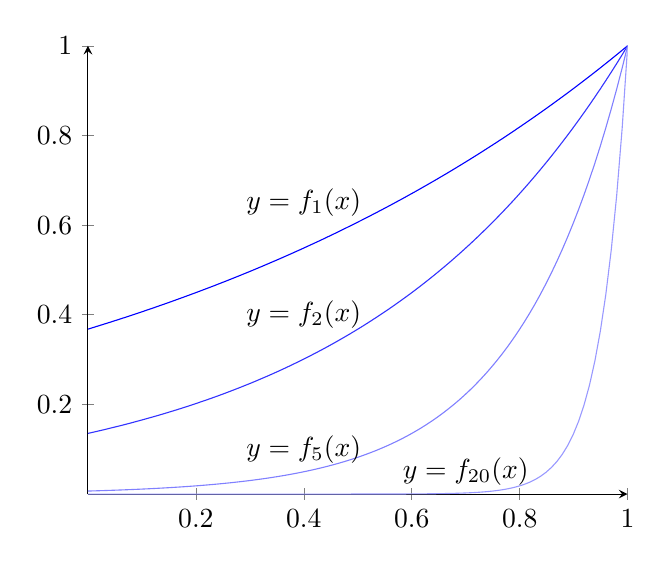
\begin{tikzpicture}
        \begin{axis}[axis lines=center]
            \addplot[
                domain=0:1,
                samples=100,
                color=blue,
            ] {exp(x-1)};
            \addplot[
                domain=0:1,
                samples=100,
                color=blue!80,
            ] {exp(2*x-2)};
            \addplot[
                domain=0:1,
                samples=100,
                color=blue!50,
            ] {exp(5*x-5)};
            \addplot[
                domain=0:1,
                samples=100,
                color=blue!40,
            ] {exp(20*x-20)};
            
            \node at (axis cs:0.4, 0.65) {$y = f_1(x)$};
            \node at (axis cs:0.4, 0.4) {$y = f_2(x)$};
            \node at (axis cs:0.4, 0.1) {$y = f_5(x)$};
            \node at (axis cs:0.7, 0.05) {$y = f_{20}(x)$};
        \end{axis}
    \end{tikzpicture}
\end{figure}
\noindent So, the integral of the sequence of functions is tending towards $0$, i.e. $f_n \to 0$. This is because
\begin{align*}
    d_1(f_n, 0) &= \int_0^1 |f_n(x)| \ dx \\
    &= \int_0^1 e^{n(x-1)} \ dx \\
    &= \left[\frac{1}{n} e^{n(x-1)}\right]_0^1 \\
    &= \frac{1}{n} - \frac{1}{n} e^{-n} \\
    &= \frac{1}{n} (1 - e^{-n}) \to 0.
\end{align*}
However, for all $n \in \mathbb{Z}_{\geqslant 1}$, $ev(f_n) = e^{n(1-1)} = 1 \neq 0$. Therefore, the function $ev$ is not $(d_1, d_2)$-continuous.\sidefootnote{Is the function $(d_\infty, d_2)$-continuous?}

Now, we will look at another non-continuous function. Define the function $f: \mathbb{R} \to \mathbb{R}^2$ by $f(x) = (x, 1)$. The function $f$ is not $(d_2, D)$-continuous, where $D$ is the railroad metric on $\mathbb{R}^2$ at any point $a \in \mathbb{R}$. Define the sequence $(x_n)_{n=1}^{\infty}$ by $a + \frac{1}{n}$. We know that $x_n \to a$ in $\mathbb{R}$. The diagram below shows how the sequence $(f(x_n))_{n=1}^{\infty}$ approaches $f(a)$:
\begin{figure}[H]
    \centering
    \begin{tikzpicture}
        \begin{axis}[
            axis lines=center,
            ymin=0, ymax=2,
            xmin=0, xmax=2.5,
            ytick={1},
            xtick={1, 1.1, 1.25, 1.5, 2},
            xticklabels={$a$, $x_6$, $x_4$, $x_2$, $x_1$}
        ]
            \node[circle, draw, inner sep=1.5pt, blue, fill=blue!50, opacity=0.5] at (axis cs:1, 1) {};
            \node[circle, draw, inner sep=1.5pt, fill=blue!50, blue!50, opacity=0.5] at (axis cs:1.1, 1) {};
            \node[circle, draw, inner sep=1.5pt, fill=blue!50, blue!50, opacity=0.5] at (axis cs:1.25, 1) {};
            \node[circle, draw, inner sep=1.5pt, fill=blue!50, blue!50, opacity=0.5] at (axis cs:1.5, 1) {};
            \node[circle, draw, inner sep=1.5pt, fill=blue!50, blue!50, opacity=0.5] at (axis cs:2, 1) {};
        \end{axis}
    \end{tikzpicture}
\end{figure}
\noindent Clearly, $f(x_n) = (x_n, 1)$ is not collinear to $\bm{0}$ and $f(a) = (a, 1)$ for all $n \in \mathbb{Z}_{\geqslant 1}$. So, we find that
\[d(f(x_n), f(a)) = \lVert f(x_n) \rVert + \lVert f(a) \rVert \geqslant \lVert (a, 1) \rVert \geqslant 1.\]
So, $f(x_n) \not\to f(a)$ with respect to the railroad metric. So, $f$ is not $(d_2, D)$-continuous.
\newpage

\section{Cauchy Sequences and Completeness}
In this section, we will consider Cauchy sequences, and how we can define completeness from this concept. We start by generalising Cauchy sequences in metric spaces.
\begin{definition}
Let $(X, d)$ be a metric space, and let $(x_n)_{n=1}^{\infty}$ be a sequence in $X$. Then, the sequence $(x_n)$ is \emph{Cauchy} if for every $\varepsilon > 0$, there exists an $N \in \mathbb{Z}_{\geqslant 1}$ such that for $m, n \in \mathbb{Z}_{\geqslant 1}$, if $m, n \geqslant N$, then $d(x_n, x_m) < \varepsilon$.
\end{definition}
\noindent Intuitively, a sequence being Cauchy means that the values in the sequences are getting arbitrarily close to each other. In $\mathbb{R}$, every Cauchy sequence converges- we will review this proof.
\begin{theorem}
Let $(x_n)_{n=1}^{\infty}$ in $\mathbb{R}$ be a Cauchy sequence. Then, there exists an $x \in \mathbb{R}$ such that $x_n \to x$.
\end{theorem}
\begin{proof}
\hspace*{0pt}
\begin{itemize}
    \item We first show that $(x_n)_{n=1}^{\infty}$ is bounded. Since the sequence is Cauchy, there exists an $N \in \mathbb{Z}_{\geqslant 1}$ such that for all $m, n \in \mathbb{Z}_{\geqslant 1}$, if $m, n \geqslant N$, then $|x_n - x_m| < 1$. In particular, for all $n \in \mathbb{Z}_{\geqslant 1}$, $|x_n - x_N| < 1$, and so 
    \[|x_n| \leqslant |x_n - x_N| + |x_N| = 1 + |x_N|.\]
    This implies that
    \[K = \max (|x_1|, |x_2|, \dots, |x_N|) + 1\]
    is a bound for the sequence- for all $i \in \mathbb{Z}_{\geqslant 1}$, if $i \leqslant N$, $|x_i| < K$ by construction; and for $i > N$, we have $|x_i| \leqslant 1 + |x_N| < K$.
    
    \item Now, the Bolzano-Weierstrass theorem tells us that $(x_n)$ has a convergent subsequence $x_{k_n} \to x$.
    
    \item Finally, we show that $x_n \to x$. Let $\varepsilon > 0$. Since $x_{k_n} \to x$, there exists an $N_1 \in \mathbb{Z}_{\geqslant 1}$ such that for $n \in \mathbb{Z}_{\geqslant 1}$, if $n \geqslant N_1$, then $|x_{k_n} - x| < \frac{\varepsilon}{2}$. Moreover, since $(x_n)$ is Cauchy, there exists an $N_2 \in \mathbb{Z}_{\geqslant 1}$ such that for $m, n \in \mathbb{Z}_{\geqslant 1}$, if $m, n \geqslant N_2$, then $|x_n - x_m| < \frac{\varepsilon}{2}$. So, set $N = \max(N_1, N_2)$. In that case, for $n \in \mathbb{Z}_{\geqslant 1}$, if $n \geqslant N$, then we have $k_n \geqslant n \geqslant N$. This implies that
    \begin{align*}
        |x_n - x| &= |x_n - x_{k_n} + x_{k_n} - x| \\
        &\leqslant |x_n - x_{k_n}| + |x_{k_n} - x| \\
        &< \frac{\varepsilon}{2} + \frac{\varepsilon}{2} = \varepsilon.
    \end{align*}
    This implies that $x_n \to x$.
\end{itemize}
\end{proof}
\noindent Although this is not true for every metric space, i.e. not every Cauchy sequence converges, it is true that every convergent sequence is Cauchy.
\begin{proposition}
Let $(X, d)$ be a metric space, and let $(x_n)_{n=1}^{\infty}$ be a convergent sequence in $X$. Then, $(x_n)$ is Cauchy.
\end{proposition}
\begin{proof}
Assume that $x_n \to x$ for some $x \in X$. Let $\varepsilon > 0$. Since $(x_n)$ is convergent, there exists an $N \in \mathbb{Z}_{\geqslant 1}$ such that for $n \in \mathbb{Z}_{\geqslant 1}$, if $n \geqslant N$, then $d(x_n, x) < \frac{\varepsilon}{2}$. In that case, for $m, n \in \mathbb{Z}_{\geqslant 1}$, if $m, n \geqslant N$, then
\[d(x_m, x_n) \leqslant d(x_m, x) + d(x, x_n) < \frac{\varepsilon}{2} + \frac{\varepsilon}{2} = \varepsilon.\]
This implies that the sequence $(x_n)$ is Cauchy.
\end{proof}

Now, we will look at some Cauchy sequences that do not converge. We know that $\pi \in \mathbb{R}$ is not rational. So, let $X = \mathbb{Q}$ with the subspace metric from $\mathbb{R}$, and let $(x_n)_{n=1}^{\infty}$ be the decimal expansion of $\pi$ up to $n$ digits, i.e.
\[x_1 = 3.1, \qquad x_2 = 3.14, \qquad x_3 = 3.141, \qquad x_4 = 3.1415, \qquad \dots.\]
As the sequence in $\mathbb{R}$ converges to $\pi$, the sequence is Cauchy in $\mathbb{R}$. As $(x_n)$ is a sequence in $\mathbb{Q}$, it is also Cauchy in $\mathbb{Q}$. However, it is not convergent since $\pi \not\in \mathbb{Q}$, and limits are unique. That is, if $x_n \to a$ in $\mathbb{Q}$ and $x_n \to b$ in $\mathbb{R}$, $a = b$. This is because the Euclidean metric coincides with the subspace metric for every pair of points in $\mathbb{Q}$. So, there are many metric spaces that are Cauchy sequences but not convergent. 

Now, we will define completeness.
\begin{definition}
Let $(X, d)$ be a metric space. Then, $X$ is \emph{complete} if for every sequence $(x_n)_{n=1}^{\infty}$ in $X$, if $(x_n)$ is Cauchy, then $(x_n)$ is convergent in $X$.
\end{definition}
\noindent We have seen that $\mathbb{Q}$ is not a complete metric space. Moreover, $\mathbb{R}$ is a complete metric space. Similarly, $\mathbb{R}^n$ is a complete metric space under $d_1$ and $d_\infty$ metric- this is because a sequence $(x_{11}, x_{12}, \dots, x_{1n})_{i=1}^{\infty}$ converges in $\mathbb{R}^n$ to $(y_1, y_2, \dots, y_n)$ if and only if $x_i \to y_i$ in $\mathbb{R}$ for all $i \in \{1, 2, \dots, n\}$. 

Now, we will look at a general example of a complete metric space. Let $X$ be a non-empty set, and let $d$ be the discrete metric space. We show that $(X, d)$ is complete. To see this, let $(x_n)_{n=1}^{\infty}$ be a Cauchy sequence in $X$. In that case, there exists an $N \in \mathbb{Z}_{\geqslant 1}$ such that for $m, n \in \mathbb{Z}_{\geqslant 1}$, if $m, n \geqslant N$, then $d(x_m, x_n) < 1$. In particular, for $n \in \mathbb{Z}_{\geqslant 1}$, if $n \geqslant N$, then $d(x_n, x_N) < 1$. Since $d$ is the discrete metric, this implies that $x_n = X_N$. Therefore, for all $n \geqslant N$, $x_n = x_N$. So, the sequence $x_n \to x_N$- the sequence is convergent. This also illustrates that completeness depends on the metric we choose- $\mathbb{Q}$ is complete under the discrete metric, and not complete under the Euclidean subspace metric.

We will now show that complete sequences satisfy the Contraction Mapping Theorem. To state this, we need to define some concepts.
\begin{definition}
Let $(X, d)$ be a metric space, and let $T: X \to X$ be a function. Then, $x_0 \in X$ is a \emph{fixed point of $T$} if $f(x_0) = x_0$.
\end{definition}
\begin{definition}
Let $(X, d)$ be a metric space, and let $T: X \to X$ be a function. Then, $T$ is a \emph{contraction} if there exists a $0 < c < 1$ such that $d(T(x), T(y)) < cd(x, y)$ for all $x, y \in X$ with $x \neq y$.
\end{definition}
\noindent Intuitively, the function moves all the points closer. Using these definitions, we state the theorem.
\begin{theorem}[Contraction Mapping Theorem]
Let $(X, d)$ be a complete metric space, and let $T: X \to X$ be a contraction. Then, $T$ has a unique fixed point.
\end{theorem}
\begin{proof}
\hspace*{0pt}
\begin{itemize}
    \item We first show that $T$ has a fixed point. Let $x_0 \in X$. Define the sequence $(x_n)_{n=1}^{\infty}$ in $X$ by $x_1 = T(x_0)$ and $x_{n+1} = T(x_n)$. We show that $(x_n)$ is Cauchy.
    \begin{itemize}
        \item First, we show that for all $n \in \mathbb{Z}_{\geqslant 1}$, $d(x_{n+1}, x_n) < c^n d(x_1, x_0)$, where $c \in (0, 1)$ is the contraction constant for $T$. We know that 
        \[d(x_2, x_1) = d(T(x_1), T(x_0)) < cd(x_1, x_0),\]
        so the statement is true if $n = 1$. Now, if $d(x_{n+1}, x_n) < c^n d(x_1, x_0)$ for some $n \in \mathbb{Z}_{\geqslant 1}$, then
        \begin{align*}
            d(x_{n+2}, x_{n+1}) &= d(T(x_{n+1}), T(x_n)) \\
            &< cd(x_{n+1}, x_n) \\
            &< c \cdot c^n d(x_1, x_0) = c^{n+1} d(x_1, x_0).
        \end{align*}
        Therefore, the statement holds for all $n \in \mathbb{Z}_{\geqslant 1}$ by induction.
        
        \item Using this, we show that $(x_n)$ is Cauchy. Let $\varepsilon > 0$. For $m, n \in \mathbb{Z}_{\geqslant 1}$, with $n \geqslant m$, we find that
        \begin{align*}
            d(x_n, x_m) &\leqslant d(x_n, x_{n-1}) + d(x_{n-1}, x_m) \\
            &\leqslant d(x_n, x_{n-1}) + d(x_{n-1}, x_{n-2}) + \dots + d(x_{m+1}, x_m) \\
            &< c^{n-1} d(x_1, x_0) + c^{n-2} d(x_1, x_0) + c^m (x_1, x_0) \\
            &= c^m d(x_1, x_0) [c^{n-1} + \dots + c + 1] \\
            &\leqslant c^m d(x_1, x_0) \cdot \sum_{i=0}^\infty c^i \\
            &= \frac{c^m}{1 - c} d(x_1, x_0).
        \end{align*}
        So, choose $N \in \mathbb{Z}_{\geqslant 1}$ such that $c^N < \frac{d(x_1, x_0)}{(1-c) \varepsilon}$- this is possible since $c \in (0, 1)$. Then, for all $m, n \in \mathbb{Z}_{\geqslant 1}$, if $n \geqslant m \geqslant 1$, then
        \[d(x_n, x_m) \leqslant \frac{c^m}{1 - c} d(x_1, x_0) \leqslant \frac{c^N}{1-c} d(x_1, x_0) < \varepsilon.\]
        Therefore, the sequence $(x_n)$ is Cauchy.
    \end{itemize}
    Since $X$ is complete, we find that $x_n \to x$, for some $x \in X$. Moreover, $T(x_n) = x_{n+1} \to x$. This implies that $T(x) = x$, so $x$ is a fixed point of $T$.
    
    \item We now show that the fixed point is unique. Let $x_1, x_2 \in X$ such that $T(x_1) = x_1$ and $T(x_2) = x_2$. In that case, if $x_1 \neq x_2$, then
    \[d(x_1, x_2) = d(T(x_1), T(x_2)) < cd(x_1, x_2).\]
    This is not possible, so we must have $x_1 = x_2$. Therefore, the fixed point is unique.
\end{itemize}
\end{proof}
\noindent We now look at an explicit example of this theorem. Take $X = [\frac{3}{2}, \infty)$ with the subspace metric from $\mathbb{R}$. We will see later that $X$ is complete. Define the function $T: X \to X$ by $T(x) = \frac{1}{2}(x + \frac{3}{x})$. We claim that $T$ is a contraction, with unique fixed point $\sqrt{3}$. Let $x, y \in X$ with $x \neq y$,
\begin{align*}
    |T(x) - T(y)| &= \frac{1}{2} \left|x + \frac{3}{x}  - y - \frac{3}{y}\right| \\
    &= \frac{1}{2}|x-y| \left|1 - \frac{3}{xy}\right| \\
    &< \frac{1}{2}|x-y|,
\end{align*}
since for $x, y \in [\frac{3}{2}, \infty)$, $|1 - \frac{3}{xy}| < 1$. Therefore, $T$ is a contraction. Moreover,
\[T(\sqrt{3}) = \frac{1}{2} \left(\sqrt{3} + \frac{3}{\sqrt{3}}\right) = \sqrt{3},\]
so $\sqrt{3}$ is a fixed point. The Contraction Mapping Theorem tells us that $\sqrt{3}$ is the unique fixed point.

Next, we look at applications of the Contraction Mapping Theorem. It is used in the proof of the Inverse Function Theorem; proof of the existence and uniqueness of solutions to ODEs; and it is used in population dynamics.

\newpage

\section{Open and Closed Sets}
\subsection{Open Sets}
In this section, we define open and closed sets. We have already defined open balls in a metric space- these are open sets. We generalise this to open sets.
\begin{definition}
Let $(X, d)$ be a metric space. A subset $U \subseteq X$ is \emph{open} if for every $x \in U$, there exists an $r > 0$ such that $B_X(x, r) \subseteq U$.
\end{definition}
\noindent So, for a subset $U$ to be open, every element $x \in U$ must have some open ball around it so that the open ball is contained in $U$- the `boundary' of $U$ is not contained in $U$. For example, the value $x$ is not in the boundary of the open ball in the figure below.
\begin{figure}[H]
    \centering
    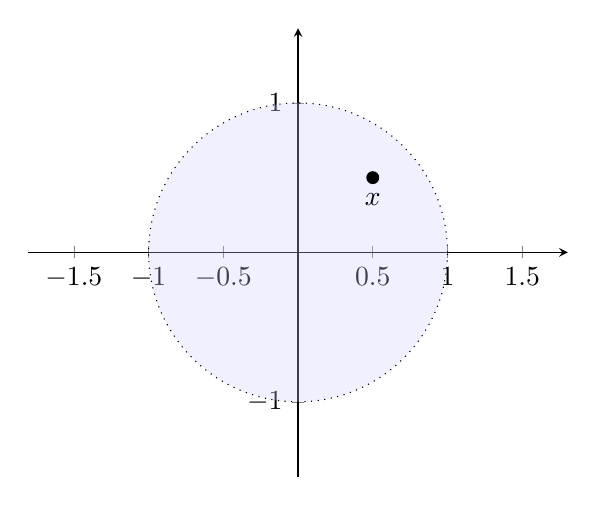
\begin{tikzpicture}
        \begin{axis}[
            axis lines=center,
            ymin=-1.5, ymax=1.5,
            xmin=-1.5, xmax=1.5,
            axis equal,
        ]
            \fill[fill=blue!20, opacity=0.3] (axis cs:0, 0) circle (1);
            \draw[dotted] (axis cs:0, 0) circle (1);
            \node[circle, draw, inner sep=1.5pt, fill=black, label={-90:$x$}] at (axis cs: .5, .5) {};
        \end{axis}
    \end{tikzpicture}
\end{figure}
Now, we will look at some examples of open sets. Let $(X, d)$ be a metric space. Then, both $X$ and the empty set $\varnothing$ are open in $X$. The argument is vacuous for the empty set- there are no points in the empty set. For $X$, take $x \in X$. By construction, $B_X(x, 1) \subseteq X$. Therefore, $X$ is open. Next, an interval of the form 
\[(a, b) = \{x \in \mathbb{R} \mid a < x < b\} \subseteq \mathbb{R}\]
is open in Euclidean metric. To see this, let $x \in (a, b)$. Set $r = \frac{1}{2} \min(x - a, b - x) > 0$. Then,
\[x - r \geqslant x - \frac{1}{2}(x - a) = \frac{1}{2}(x + a) > \frac{1}{2}(a + a) = a,\]
and
\[x + r \leqslant x + \frac{1}{2}(b - x) = \frac{1}{2}(x + b) < \frac{1}{2}(b + b)= b.\]
This implies that 
\[B_{\mathbb{R}}(x, r) = (x-r, x+r) \subseteq (a, b).\]
Therefore, the interval $(a, b)$ is open. We generalise this to open balls in any metric space.
\begin{lemma}
Let $(X, d)$ be a metric space, $x \in X$ and $r > 0$. Then, the open ball around $x$ of radius $r$, $B_X(x, r)$ is an open set.
% \sidefootnote{This does not follow from the definition- we know that for all $y \in B_X(x, r)$, $d(x, y) < r$, but we need an open ball around every point in $B_X(x, r)$}
\end{lemma}
\begin{proof}
Let $y \in B_X(x, r)$. By definition, we find that $d(x, y) < r$. Set $\varepsilon = r - d(x, y) > 0$. We claim that $B_X(y, \varepsilon) \subseteq B_X(x, r)$. Let $z \in B_X(y, \varepsilon)$. So, $d(y, z) < \varepsilon$. In that case,
\[d(x, z) \leqslant d(x, y) + d(y, z) = r - \varepsilon + d(y, z) < r.\]
So, $z \in B_X(z, r)$. This implies that $B_X(y, \varepsilon) \subseteq B_X(x, r)$.
\end{proof}

Now, take $X = \mathbb{R}^2$ with the Euclidean metric, and define the square $U = (-2, 0) \times (1, 3)$
\[\{(x, y) \in \mathbb{R}^2 \mid -2 < x < 0, 1 < y < 3\}.\]
Then, the set $U$ is open. The interval is highlighted in the figure below.
\begin{figure}[H]
    \centering
    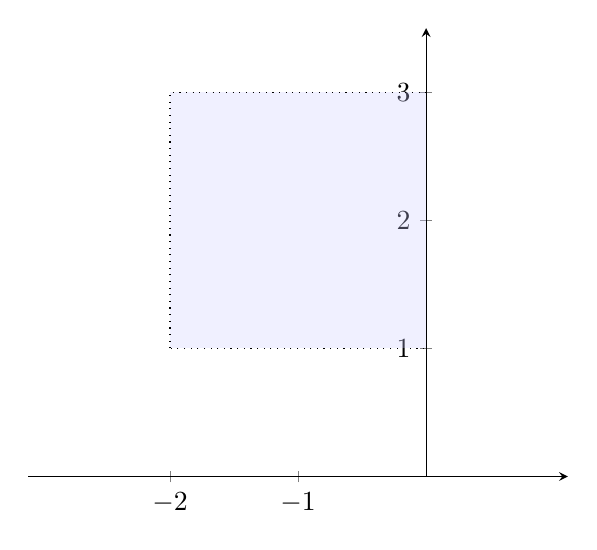
\begin{tikzpicture}
        \begin{axis}[
            axis lines=center,
            xmin=-2.5, xmax=.5,
            ymin=0, ymax=3.5,
            xtick={-2, -1, 0},
            axis equal,
        ]
            \fill[fill=blue!20, opacity=0.3] (axis cs:-2, 1) -- (axis cs:-2, 3) -- (axis cs:0, 3) -- (axis cs:0, 1) -- cycle;
            \draw[dotted] (axis cs:-2, 1) -- (axis cs:-2, 3) -- (axis cs:0, 3) -- (axis cs:0, 1) -- cycle;
        \end{axis}
    \end{tikzpicture}
\end{figure}
\noindent To prove this, let $(x, y) \in U$. Let $r = \frac{1}{2} \min(x+2, -x, y-1, 3-y)$. In that case, $(x + r, x - r) \subseteq (-2, 0)$ and $(y-r, y+r) \subseteq (1, 3)$. We use this result to show that $B_{\mathbb{R}^2}((x, y), r) \subseteq U$. So, let $z \in B_{\mathbb{R}^2}((x, y), r)$. We find that 
\[|x - z_1| \leqslant \sqrt{(x - z_1)^2 + (y - z_2)^2} < r,\]
and
\[|y - z_2| \leqslant \sqrt{(x - z_1)^2 + (y - z_2)^2} < r.\]
Therefore, $z_1 \in (x - r, x + r)$ and $z_2 \in (y - r, y + r)$. So, 
\[z \in (x - r, x + r) \times (y-r, y+r) \subseteq U.\]
This implies that $U$ is an open set.

We now look at another example. Let $(X, d)$ be a metric space, let $x \in X$ and $r > 0$. Then,
\[U = \{y \in X \mid d(x, y) > r\}\]
is open. To see this, let $a \in U$. We know that $d(x, a) > r$. Let $\varepsilon = d(x, a) - r > 0$. We claim that the open ball $B_X(a, \varepsilon) \subseteq U$. So, let $z \in B_X(a, \varepsilon)$. Then, $d(a, z) < \varepsilon$. In that case,
\[r + \varepsilon = d(x, a) \leqslant d(x, z) + d(z, a) < d(x, z) + \varepsilon.\]
So, $d(x, z) > r$ . This implies that $z \in U$. Therefore, $B_X(a, \varepsilon) \subseteq U$, meaning that $U$ is open.

Now, we show that arbitrary unions of open sets is open.
\begin{proposition}
Let $(X, d)$ be a metric space, $I$ be an indexing set, and $(U_i)_{i \in I}$ be a collection of open sets in $X$. Then, the union
\[U = \bigcup_{i \in I} U_i\]
is open in $X$.
\end{proposition}
\begin{proof}
Let $x \in U$. By definition, there exists an $i \in I$ such that $x \in U_i$. Since $U_i$ is open, there exists an $r > 0$ such that
\[B_X(x, r) \subseteq U_i \subseteq U.\]
This implies that $U$ is open in $X$.
\end{proof}
\noindent Next, we show that finite intersection of open sets is open.
\begin{proposition}
Let $(X, d)$ be a metric space, and $U_1, \dots, U_n$ be open sets in $X$. Then, the intersection
\[I = \bigcap_{i=1}^n U_i\]
is open in $X$.
\end{proposition}
\begin{proof}
Let $x \in I$. Since $U_i$ is open for every $i \in \{1, 2, \dots, n\}$, there exists an $r_i > 0$ such that $B_X(x, r_i) \subseteq U_i$. Now, set
\[r = \min(r_1, r_2, \dots, r_n) > 0.\]
We find that $B_X(x, r) \subseteq B_X(x, r_i) \subseteq U_i$ for all $i \in \{1, 2, \dots, n\}$. Therefore, $B_X(x, r) \subseteq I$. This implies that $I$ is open in $X$.
\end{proof}
\noindent The finiteness is required in this proof since we have to take the minimum. It is not true, in general, that an infinite intersection of open sets is open. For example, let $X = \mathbb{R}$ with the Euclidean metric. Define the subset $U_n = (-\frac{1}{n}, \frac{1}{n})$ for $n \in \mathbb{Z}_{\geqslant 1}$. Each of these subsets is an open interval, so it is open in $\mathbb{R}$. We know that $0 \in (-\frac{1}{n}, \frac{1}{n})$ for all $n \in \mathbb{Z}_{\geqslant 1}$. In fact,
\[I = \bigcap_{i=1}^n U_n = \{0\}.\]
This is because, for $x \neq 0$, we can find an $n \in \mathbb{Z}_{\geqslant 1}$ such that $n > \frac{1}{|x|}$, and so $x \not\in (\frac{-1}{n}, \frac{1}{n})$. However, the set $\{0\}$ is not open in $\mathbb{R}$. This is because, for all $r > 0$, $B_{\mathbb{R}}(0, r) = (-r, r) \not\subseteq \{0\}$ since $\frac{r}{2} \in (-r, r)$ but $\frac{r}{2} \neq 0$.

Next, let $X = \mathbb{R}^2$ with the Euclidean metric $d_2$. For $n \in \mathbb{Z}_{\geqslant 1}$, define
\[U_n = \{(x, y) \in \mathbb{R}^2 \mid -\tfrac{4}{n^2} < y < \tfrac{3}{n^2}\}.\]
We claim that $U_n$ is open. Let $(x, y) \in U_n$. Set $\varepsilon = \min(y + \frac{4}{n^2}, \frac{3}{n^2} - y)$. Then, 
\begin{align*}
    B_{\mathbb{R}^2}((x, y), r) &= \{(r, s) \in \mathbb{R}^2 \mid \sqrt{(r-x)^2 + (s-y)^2} < \varepsilon\} \\
    &\subseteq \{(r, s) \in \mathbb{R}^2 \mid |s-y| < \varepsilon\} \subseteq U_n.
\end{align*}
% TODO: Justify |s-y| < r => (r, s) \in U_n
\noindent Therefore, $U_n$ is open. Moreover, the intersection
\[I = \bigcap_{i=1}^n U_i = \mathbb{R} \times \{0\}\]
is not open in $\mathbb{R}^2$. This is because, for all $r > 0$, 
\[B_{\mathbb{R}^2}((0, 0), r) = \{(x, y) \in \mathbb{R}^2 \mid \sqrt{x^2 + y^2} < r\} \not\subseteq \mathbb{R} \times \{0\},\]
since $(0,r) \in B_{\mathbb{R}^2}((0, 0), r)$ but $(0, r) \not\in \mathbb{R} \times \{0\}$.

\subsection{Closed Sets}
Now, we look at closed sets.
\begin{definition}
Let $(X, d)$ be a metric space and $C \subseteq X$. Then, $U$ is \emph{closed} if its complement $X \setminus C$ is open.
\end{definition}
\noindent So, the `opposite' of open sets is closed. However, the relation between open and closed sets is not that simple. For instance, the sets $X$ and $\varnothing$ are closed- this is because $X$ and $\varnothing$ are open, and complement of each other. So, there can be sets that are both open and closed.

Now, if $(X, d)$ is a metric space, then the closed ball of radius $r > 0$ around $x \in X$,
\[\overline{B}_X(x, r) = \{y \in X \mid d(x, y) \leqslant r\}\]
is closed. This is because its complement is
\[U = \{y \in X \mid d(x, y) > r\},\]
which we have shown to be open. 

Next, let $V \subseteq X$ be finite. Then, $V$ is closed. If $X = V$, then we know that $V$ is closed. So, assume that $X \neq V$, i.e. the complement $U = X \setminus V$ is non-empty. So, let $u \in U$. Define
\[r = \min_{v \in V} d(v, u).\]
Since $V$ is finite, the minimum exists. Moreover, since $u \not\in V$, $r > 0$. Then, by definition, for all $v \in V$, $d(v, u) \geqslant r$. So, $v \not\in B_X(u, r)$ for all $v \in V$. Therefore, the intersection $B_X(u, r) \cap V = \varnothing$. In that case, $B_X(u, r) \subseteq U$. This implies that $V$ is closed.

\subsection{Open sets in subspaces}
Now, we will look at open sets in subspaces, i.e. with the subspace metric. So, let $(X, d)$ be a metric space and $(A, d_A)$ be the subspace metric, for some $A \subseteq X$. For $a \in A$ and $r > 0$, the open ball
\begin{align*}
    B_A(a, r) &= \{b \in A \mid d_A(a, b) < r\} \\
    &= \{b \in A \mid d(a, b) < r\} \\
    &= \{x \in X \mid d(a, x) < r\} \cap A \\
    &= B_X(a, r) \cap A.
\end{align*}
In fact, a general open set in $A$ is of the form the intersection of $A$ and some open set in $X$.
\begin{proposition}
Let $(X, d)$ be a metric space and let $A \subseteq X$. Then, a subset $U \subseteq A$ is open in $A$ if and only if $U = V \cap A$, for some subset $V \subseteq X$ that is open in $X$.
\end{proposition}
\begin{proof}
\hspace*{0pt}
\begin{itemize}
    \item First, assume that $U = V \cap A$, where $V$ is open in $X$. Let $a \in U$. Since $a \in V$ and $V$ is open, there exists an $r > 0$ such that $B_X(a, r) \subseteq V$. In that case,
    \[B_A(a, r) = B_X(a, r) \cap A \subseteq V \cap A \subseteq U.\]
    This implies that $U$ is open in $A$.
    
    \item Now, assume that $U$ is open in $A$. In that case, for each $u \in U$, there exists an $r_u > 0$ such that the open ball $B_A(u, r_u) \subseteq U$. We know that
    \[U = \bigcup_{u \in U} B_A(u, r_u).\]
    This is because for all $u \in U$, $u \in B_A(u, r_u)$. Now, denote
    \[V = \bigcup_{u \in U} B_X(u, r_u).\]
    We know that $B_X(u, r_u)$ is open in $X$ for all $u \in U$, so the union $V$ will also be open in $X$. Moreover, we show that $V \cap A = U$.
    \begin{itemize}
        \item First, if $u \in U$, then $u \in B_X(u, r_u) \subseteq V$. Furthermore, since $u \in A$, we find that $u \in V \cap A$.
        
        \item Now, if $v \in V \cap A$, then $v \in V$. This implies that there exists a $u \in U$ such that $v \in B_X(u, r_u)$. Moreover, since $v \in A$, we find that
        \[v \in B_X(u, r_u) \cap A = B_A(u, r_u).\]
        Moreover, $B_A(u, r_u) \subseteq U$ by construction. This implies that $v \in U$.
    \end{itemize}
    Therefore, $V \cap A = U$.
\end{itemize}
This implies that $U \subseteq A$ is open in $A$ if and only if $U = V \cap A$, for some subset $V \subseteq X$ that is open in $X$.
\end{proof}
\noindent For instance, let $X = \mathbb{R}$ and $A = (-1, 4]$. Then, the open balls in $A$ are all of the form $(x - r, x + r) \cap (-1, 4]$, for some $x \in A, r > 0$. Moreover, any open set in $A$ is the union of these open balls.

\subsection{Continuity and Open Sets}
Now, we characterise continuity using open sets.
\begin{proposition}
Let $(X, d_X)$ and $(Y, d_Y)$ be metric spaces and let $f: X \to Y$ be a function. Then, $f$ is $(d_x, d_Y)$-continuous if and only if for every open set $U \subseteq Y$, its preimage
\[f^{-1}(U) = \{x \in X \mid f(x) \in U\}\]
is open in $X$.
\end{proposition}
\begin{proof}
\hspace*{0pt}
\begin{itemize}
    \item First, assume that $f$ is $(d_X, d_Y)$-continuous. Let $U \subseteq Y$ be open in $Y$, and let $x \in f^{-1}(U)$. Since $f(x) \in U$ and $U$ is open in $Y$, there exists an $\varepsilon > 0$ such that $B_Y(f(x), \varepsilon) \subseteq U$. Moreover, since $f$ is continuous, there exists a $\delta > 0$ such that 
    \[f(B_X(x, \delta)) \subseteq B_Y(f(X), \varepsilon) \subseteq U.\]
    Therefore, for all $x_0 \in B_X(x, \delta)$, $f(x_0) \in U$. This implies that $B_X(x, \delta) \subseteq f^{-1}(U)$. So, the set $f^{-1}(U)$ is open in $X$.
    
    \item Now, assume that for every open set $U \subseteq Y$, its preimage $f^{-1}(U)$ is open in $X$. Let $x \in X$ and $\varepsilon > 0$. We know that the set $U = B_Y(f(x), \varepsilon)$ is open. Therefore, its preimage $f^{-1}(U)$ is open. We have $f(x) \in U$, so $x \in f^{-1}(U)$. So, there exists a $\delta > 0$ such that $B_X(x, \delta) \subseteq f^{-1}(U)$. In that case,
    \[f(B_X(x, \delta)) \subseteq U = B_Y(f(x), \varepsilon).\]
    This implies that $f$ is continuous.
\end{itemize}
So, $f$ is $(d_X, d_Y)$-continuous if and only if for every open set $U \subseteq Y$, its preimage $f^{-1}(U)$ is open in $X$.
\end{proof}
\noindent There is an equivalent proposition in terms of closed sets.
\begin{corollary}
Let $(X, d_X)$ and $(Y, d_Y)$ be metric spaces and let $f: X \to Y$ be a function. Then, $f$ is $(d_X, d_Y)$-continuous if and only if for every closed set $U \subseteq Y$, its preimage $f^{-1}(U)$ is closed in $X$.
\end{corollary}
% TODO: Prove it, idk?
\noindent This follows from the definition of closed sets- a closed set is the complement of some open set.

We will use these results to prove that sets are open/closed. We know that a polynomial function $p: \mathbb{R}^n \to \mathbb{R}$ is $(d_2, d_2)$-continuous. Therefore, the functions $f, g: \mathbb{R}^2 \to \mathbb{R}$ given by $f(x, y) = x$ and $g(x, y) = y$ are continuous. Let $a, b, c, d \in \mathbb{R}$ with $a < b$ and $c < b$. We show that the set $(a, b) \times (c, d)$ is open in $\mathbb{R}^2$. We know that the sets $(a, b)$ and $(c, d)$ are open. In that case,
\begin{align*}
    V_1 &= f^{-1}((a, b)) = \{(x, y) \in \mathbb{R}^2 \mid a < x < b\} \\
    V_2 &= g^{-1}((c, d)) = \{(x, y) \in \mathbb{R}^2 \mid c < y < d\} 
\end{align*}
are open in $\mathbb{R}^2$. In that case, their intersection
\[V_1 \cap V_2 = \{(x, y) \in \mathbb{R}^2 \mid a < x < b, c < y < d\} = (a, b) \times (c, d)\]
is open in $\mathbb{R}^2$.

Now, let
\[A = \{(x, y) \in \mathbb{R}^2 \mid 1 < x^2 + y^2 < 4\}.\]
Pictorially, it is the following set.
\begin{figure}[H]
    \centering
    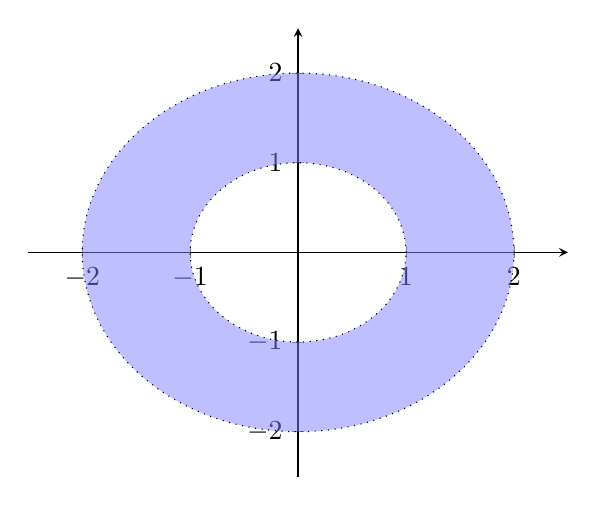
\begin{tikzpicture}
        \begin{axis}[
            axis lines=center,
            xmin=-2.5, xmax=2.5,
            ymin=-2.5, ymax=2.5,
            xtick={-2, -1, 0, 1, 2},
            ytick={-2, -1, 0, 1, 2},
        ]
            \fill [blue!50, opacity=0.5, even odd rule] (axis cs:0,0) circle[radius=2] circle[radius=1];
            \draw[black, dotted] (axis cs:0, 0) circle[radius=2];
            \draw[black, dotted] (axis cs:0, 0) circle[radius=1];
        \end{axis}
    \end{tikzpicture}
\end{figure}
\noindent We will show that this set is open in $\mathbb{R}^2$. Define the function $p: \mathbb{R}^2 \to \mathbb{R}$ by $p(x, y) = x^2 + y^2$. We note that $p$ is continuous. Since $(1, 4)$ is an open ball in $\mathbb{R}$, we find that the preimage
\[p^{-1}((1, 4)) = \{(x, y) \in \mathbb{R}^2 \mid 1 < p(x) < 4\}\]
is open.

Next, let
\[C = \{(x, y) \in \mathbb{R}^2 \mid y = x + 2\}.\]
Pictorially, it is the following set.
\begin{figure}[H]
    \centering
    \begin{tikzpicture}
        \begin{axis}[
            axis lines=center,
            xmin=-4, xmax=2,
            ymin=-2, ymax=4,
            xtick={-4, -2, 0, 2},
            ytick={-2, 0, 2, 4},
        ]
            \addplot[
                samples=100,
                domain=-4:2,
                blue
            ]{x+2};
        \end{axis}
    \end{tikzpicture}
\end{figure}
\noindent We will show that this set is closed in $\mathbb{R}^2$. Define the function $q: \mathbb{R}^2 \to \mathbb{R}$ by $q(x, y) = y - x$. Since $\{2\}$ is a closed set in $\mathbb{R}$ (it is finite), we find that the preimage
\[q^{-1}(\{2\}) = \{(x, y) \in \mathbb{R}^2 \mid q(y) = 2\}\]
is closed. 

In general, it is not true that the image of an open set under a continuous function is open. Similarly, the image of a closed set under a continuous function need not be closed. If the image of every open set is open under a continuous function $f$, then we say that $f$ is open.

\subsection{Strong Equivalence and Open Balls}
An open set in some metric is still open in another strongly equivalent metric. To show this, we start with a lemma.
\begin{lemma}
Let $(X, d_1)$ and $(X, d_2)$ be metric spaces such that there exists a $c > 0$ such that for all $x, y \in X$,
\[d_1(x, y) \leqslant cd_2(x, y).\]
Moreover, let $U \subseteq X$ be open with respect to $d_1$. Then, $U$ is open with respect to $d_2$.
\end{lemma}
\begin{proof}
Let $x \in U$. Since $U$ is open with respect to $d_1$, there exists an $r > 0$ such that $B_{(X, d_1)}(x, r) \subseteq U$. In that case, for all $y \in X$, if $d_1(x, y) < r$, then $y \in U$. Therefore, for all $y \in X$, if $d_2(x, y) < \frac{r}{c}$, then
\[d_1(x, y) \leqslant cd_2(x, y) < c \cdot \frac{r}{c} = r,\]
and so $y \in U$. Therefore, $B_{(X, d_2)}(X, \frac{r}{c}) \subseteq U$. So, $U$ is open with respect to $d_2$.
\end{proof}
\noindent Using this result, we show that strongly equivalent metrics have the same set of open sets.
\begin{proposition}
Let $(X, d_1)$ and $(X, d_2)$ be strongly equivalent metric spaces, and let $U \subseteq X$. Then, $U$ is open with respect to $d_1$ if and only if $U$ is open with respect to $d_2$.
\end{proposition}

% Strong equivalence => ..
We will now define topological equivalence.
\begin{definition}
Let $(X, d_1)$ and $(X, d_2)$ be metric spaces. Then, the metrics $d_1$ and $d_2$ are \emph{topologically equivalent} if a subset $U \subseteq X$ is open with respect to $d_1$ if and only if $U$ is open with respect to $d_2$.
\end{definition}
\noindent So, strongly equivalent metrics are topologically equivalent. In particular, the metrics $d_1$, $d_2$ and $d_\infty$ in $\mathbb{R}^2$ are topologically equivalent. Nonetheless, not every topologically equivalent metric is strongly equivalent.

\begin{lemma}
Let $(X, d_1)$, $(X, d_2)$ and $(Y, d_Y)$ be metric spaces such that $d_1$ and $d_2$ are topologically equivalent, and let $f: X \to Y$ and $g: Y \to X$ be functions. Then, 
\begin{itemize}
    \item $f$ is $(d_1, d_Y)$-continuous if and only if $f$ is $(d_2, d_Y)$-continuous;
    \item $g$ is $(d_Y, d_1)$-continuous if and only if $g$ is $(d_Y, d_2)$-continuous.
\end{itemize}
\end{lemma}
\begin{proof}
\hspace*{0pt}
\begin{itemize}
    \item \begin{itemize}
        \item Assume that $f$ is $(d_1, d_Y)$-continuous, and let $V \subseteq Y$ be open. Since $f$ is $(d_1, d_Y)$-continuous, we know that the preimage $f^{-1}(V)$ is open in $(X, d_1)$. Since $d_1$ and $d_2$ are topologically equivalent, this implies that $f^{-1}(Y)$ is open in $(X, d_2)$. Therefore, $f$ is $(d_2, d_Y)$-continuous.
        
        \item Assume that $f$ is $(d_2, d_Y)$-continuous, and let $V \subseteq Y$ be open. Since $f$ is $(d_2, d_Y)$-continuous, we know that the preimage $f^{-1}(V)$ is open in $(X, d_2)$. Since $d_1$ and $d_2$ are topologically equivalent, this implies that $f^{-1}(Y)$ is open in $(X, d_1)$. Therefore, $f$ is $(d_1, d_Y)$-continuous.
    \end{itemize}
    
    \item \begin{itemize}
        \item Assume that $g$ is $(d_Y, d_1)$-continuous, and let $U \subseteq X$ be open in $d_1$. Since $f$ is $(d_Y, d_1)$-continuous, the preimage $f^{-1}(U)$ is open in $X$. Moreover, since $d_1$ and $d_2$ are topologically equivalent, we know that $U$ is open in $(X, d_2)$ as well. This implies that $f$ is $(d_Y, d_2)$-continuous.
        
        \item Assume that $g$ is $(d_Y, d_2)$-continuous, and let $U \subseteq X$ be open in $d_2$. Since $f$ is $(d_Y, d_2)$-continuous, the preimage $f^{-1}(U)$ is open in $X$. Moreover, since $d_1$ and $d_2$ are topologically equivalent, we know that $U$ is open in $(X, d_1)$ as well. This implies that $f$ is $(d_Y, d_1)$-continuous.
    \end{itemize}
\end{itemize}
\end{proof}

\subsection{Closed Sets and Sequences}
We start by defining the closure of $U$.
\begin{definition}
Let $(X, d)$ be a metric space, and $U \subseteq X$. Then, the \emph{closure} of $U$, denoted by $\overline{U}$, is the set of all points $a \in X$ such that there exists a sequence $(x_n)_{n=1}^{\infty}$ in $U$ with $x_n \to a$.
\end{definition}
\noindent We illustrate this with an example.
\begin{figure}[H]
    \centering
    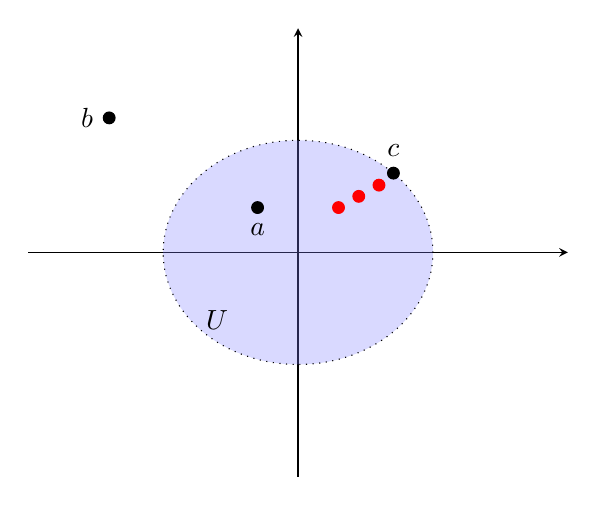
\begin{tikzpicture}
        \begin{axis}[
            axis lines=center,
            ticks=none,
            ymin=-2, ymax=2,
            xmin=-2, xmax=2,
        ]
            \fill[fill=blue!50, opacity=0.3] (axis cs: 0, 0) circle (1);
            \draw[dotted] (axis cs: 0, 0) circle (1);
            
            \node[circle, fill=black, draw, inner sep=1.5pt, label={-90:$a$}] at (axis cs:-.3, .4) {};
            \node[circle, fill=black, draw, inner sep=1.5pt, label={180:$b$}] at (axis cs:-1.4, 1.2) {};
            \node[circle, fill=black, draw, inner sep=1.5pt, label={90:$c$}] at (axis cs:0.707, 0.707) {};
            
            \node at (axis cs:-.6, -.6) {$U$};
            
            \node[circle, red, fill=red, draw, inner sep=1.5pt] at (axis cs:.3, .4) {};
            \node[circle, red, fill=red, draw, inner sep=1.5pt] at (axis cs:.45, .5) {};
            \node[circle, red, fill=red, draw, inner sep=1.5pt] at (axis cs:.6, .6) {};
        \end{axis}
    \end{tikzpicture}
\end{figure}
\noindent In the picture above, the value $a$ is in the closure $\overline{U}$. This is because, since $a \in U$, the constant sequence $(a)_{n=1}^{\infty}$ is in $U$, and satisfies $a \to a$.\sidefootnote{And, in general, for every $a \in U$, $a \in \overline{U}$.} Moreover, the value $b \not\in \overline{U}$. This is because any sequence in $U$ cannot converge to $b$- the values in the sequence will always have some strictly positive distance to $b$. However, the value $c \in \overline{U}$, even though $c \not\in U$. This is because the there is a sequence within $U$ that converges to $c$- the red points are part of the sequence.

Now, let $X = \mathbb{R}$, and let $U = (2, 4)$. Then, the closure $\overline{U} = [2, 4]$. We know that for all $x \in U$, $x \in \overline{U}$. Moreover, the sequences $(x_n)_{n=1}^{\infty}$ and $(y_n)_{n=1}^{\infty}$ given by $x_n = 2 + \frac{1}{n}$ and $y_n = 4 - \frac{1}{n}$ are in $U$, and satisfy $x_n \to 2$ and $y_n \to 4$. Furthermore, for a point $x > 4$, any sequence in $U$ will satisfy $|x_n - x| > x - 4 > 0$, and so $x_n \not\to x$, and the same is true for $x < 2$.

Moreover, if $U = [2, 4]$, then $\overline{U} = [2, 4]$. In general, the closure of a closed set is the set itself.
\begin{proposition}
Let $(X, d)$ be a metric space, and let $U \subseteq X$. Then, $U$ is closed in $X$ if and only if $\overline{U} = U$.
\end{proposition}
\begin{proof}
\hspace*{0pt}
\begin{itemize}
    \item First, assume that $U$ is closed in $X$. Let $(x_n)_{n=1}^{\infty}$ be a sequence in $U$, with $x_n \to a$, for some $a \in X$. Assume that $a \not\in U$. Since $U$ is closed, the complement $V = X \setminus U$ is open. We know that $a \in V$, so there exists an $r > 0$ such that $B_X(a, r) \subseteq V$. Since $x_n \to x$, there exists a $\delta > 0$ such that $d(x_n, a) < r$. This implies that $x_n \in U$ satisfies $x_n \in B_X(a, r) \subseteq V = X \setminus U$. This is a contradiction. So, we must have $a \in U$. Since $U \subseteq \overline{U}$ as well, we find that $\overline{U} = U$.
    
    \item Now, assume that $U$ is not closed. In that case, the complement $V = X \setminus U$ is not open. So, there exists an $x \in V$ such that for all $r > 0$, there exists a $y \not\in V$ such that $d(x, y) < r$. Since $y \not\in V$, we find that $y \in U$. So, define the sequence $(y_n)_{n=1}^{\infty}$ in $U$, where $y_n$ satisfies $d(x, y) < \frac{1}{n}$. We show that $y_n \to x$. So, let $\varepsilon > 0$. Choose an $N \in \mathbb{Z}_{\geqslant 1}$ such that $N > \frac{1}{\varepsilon}$. In that case, for $n \in \mathbb{Z}_{\geqslant 1}$, 
    \[d(y_n, x) < \frac{1}{n} \leqslant \frac{1}{N} < \varepsilon.\]
    This implies that $y_n \to x$. Since $x \not\in U$, we find that $\overline{U} \neq U$.
\end{itemize}
\end{proof}
\noindent We can use this characterisation to give another proof that a finite subset is closed.
\begin{lemma}
Let $(X, d)$ be a metric space, and let $V \subseteq X$ be finite. Then, $V$ is closed in $X$.
\end{lemma}
\begin{proof}
Denote
\[V = \{y_1, \dots, y_k\},\]
and define
\[\varepsilon = \min_{\substack{i, j=1 \\ i \neq j}}^k d(y_i, y_j) > 0.\]
Now, let $(x_n)_{n=1}^{\infty}$ be a convergent sequence in $V$, with $x_n \to x$, for some $x \in X$. We know that we can find an $N \in \mathbb{Z}_{\geqslant 1}$ such that for $n \in \mathbb{Z}_{\geqslant 1}$, if $n \geqslant N$, then $d(x_n, x) < \varepsilon$. Moreover, we know that for all $i, j \in \{1, 2, \dots, k\}$, if $d(x_i, x_j) < r$, then $x_i = x_j$. Therefore, for all $n \geqslant N$, $x_n = x$. This implies that $x = x_n \in V$. So, for every sequence $(x_n)_{n=1}^{\infty}$ in $V$ with $x_n \to x$, we have $x \in V$. This implies that $V$ is closed in $X$.
\end{proof}

We finish by showing that the closure of a set $U$ is closed, and that it is the smallest closed set containing $U$.
\begin{proposition}
Let $(X, d)$ be a metric space, and let $U \subseteq X$. Then, 
\begin{itemize}
    \item the closure $\overline{U}$ is closed in $X$;
    \item if $C \subseteq X$ is closed in $X$ with $U \subseteq C$, then $\overline{U} \subseteq C$.
\end{itemize}
\end{proposition}
\begin{proof}
\hspace*{0pt}
\begin{itemize}
    \item Let $x \in X \setminus \overline{U}$. We know that for all sequences $(x_n)_{n=1}^{\infty}$ in $U$, $x_n \not\to x$. Now, let
    \[\delta = \inf_{u \in U} d(x, u) \geqslant 0.\]
    Assume that $\delta = 0$. In that case, there exists a sequence $(x_n)_{n=1}^{\infty}$ in $U$ such that $d(x_n, x) \to 0$. Now, let $\varepsilon > 0$. Since $d(x_n, x) \to 0$, there exists an $N \in \mathbb{Z}_{\geqslant 1}$ such that for $n \in \mathbb{Z}_{\geqslant 1}$, if $n \geqslant N$, then 
    \[|d(x_n, x) - 0| = d(x_n, x) < \varepsilon.\]
    This implies that $x_n \to x$. Since $x \not\in \overline{U}$, this is a contradiction. Therefore, $\delta > 0$. We know that for all $u \in U$, $d(x, u) \geqslant \delta$, and so $u \not\in B_X(a, \delta)$. In that case, $B_X(a, \delta) \subseteq X \setminus \overline{U}$. This implies that $X \setminus \overline{U}$ is open, and so $\overline{U}$ is closed.
    
    \item Let $C \subseteq X$ be closed in $X$, with $U \subseteq C$. Since $C$ is closed, we find that $C = \overline{C}$. Now, let $x \in \overline{U}$. By definition, there exists a sequence $(x_n)_{n=1}^{\infty}$ in $U$ such that $x_n \to x$. Since $U \subseteq C$, we find that $x \in \overline{C}$. This implies that
    \[\overline{U} \subseteq \overline{C} = C.\]
\end{itemize}
\end{proof}
\noindent Using this result, we can show that the closure of a subset $U$ is the intersection of all closed sets containing $U$.
\begin{corollary}
Let $(X, d)$ be a metric space, and let $U \subseteq X$. Then, $\overline{U}$ is the intersection of all the closed sets containing $U$.
\end{corollary}
\begin{proof}
We know that for a closed set $C$ containing $U$, we have $\overline{U} \subseteq C$. Moreover, since $\overline{U}$ is a closed set containing $U$, we find that $\overline{U}$ is the intersection of all the closed sets containing $U$.
\end{proof}
Now, we look at some examples:
\begin{itemize}
    \item If $U = (-1, 4] \cup (6, 7)$, then $\overline{U} = [-1, 4] \cup [6, 7]$- this is the smallest closed set containing $U$. 
    \item If $U = (-3, -2) \cup (-1, 0) \cup (2, 3)$, then $\overline{U} = [-3, -2] \cup [-1, 0] \cup [2, 3]$. 
    \item Next, let
    \[U = \left\{-\frac{2}{n^2} \mid n \in \mathbb{Z}_{\geqslant 1}\right\}.\]
    As a sequence $-\frac{2}{n^2} \to 0$. So, $\overline{U} = U \cup \{0\}$.
    \item If
    \[A = \{(x, y) \in \mathbb{R}^2 \mid 1 < x^2 + y^2 < 9\},\]
    then the closure is
    \[\overline{A} = \{(x, y) \in \mathbb{R}^2 \mid 1 \leqslant x^2 + y^2 \leqslant 9\}.\]
    \item Now, if $U = \mathbb{Q}$, then $\overline{U} = \mathbb{R}$. This is because, for any $x \in \mathbb{R}$, there exists a sequence $(x_n)_{n=1}^{\infty}$ in $\mathbb{Q}$ such that $x_n \to x$.
    \item If $U = \mathbb{Z}$, then $\overline{U} = \mathbb{Z}$. This is because $\mathbb{Z}$ is closed.\sidefootnote{For every non-integer, there exists an open ball around it such that there is no integer in that open ball!}
\end{itemize}


\end{document}